\documentclass[11pt,oneside]{article}

\usepackage[a4paper,margin=25mm,headheight=15pt]{geometry}
\usepackage[T1]{fontenc}
\usepackage[utf8]{inputenc}
\IfFileExists{libertinus.sty}{\usepackage{libertinus}}{\usepackage{lmodern}}
\usepackage{microtype}
\usepackage{amsmath,amssymb,amsthm,mathtools,mathrsfs,bm}
% Canonical mathematical notation for active FabiusFunction LaTeX documents.
%
% This file is intentionally a plain TeX input rather than a LaTeX package.
% Every standalone document loads it by an explicit path relative to that
% document's directory; included fragments inherit the definitions from their
% root document.  Keep this file independent of document layout and metadata.
%
% Contract:
%   * one command has one mathematical meaning throughout the active corpus;
%   * names encode semantic roles rather than a document-local choice of letter;
%   * visually similar but differently normalized objects have different print;
%   * every command below is defined normatively in the notation catalogue.
%
% The active corpus excludes docs/archive/.  Historical sources may retain
% their original notation only inside an explicitly labelled quotation.

\makeatletter
\@ifundefined{mathbb}{%
  \PackageError{fabius-notation}{The amssymb package must be loaded first}%
    {Load amsmath and amssymb before inputting fabius-notation.tex.}%
}{}
\@ifundefined{operatorname}{%
  \PackageError{fabius-notation}{The amsmath package must be loaded first}%
    {Load amsmath before inputting fabius-notation.tex.}%
}{}
\makeatother

% Version stamp used by the catalogue and by static audits.
\newcommand{\FabiusNotationVersion}{2026-08-31}

% Number systems.  NaturalNumbers is explicitly the nonnegative convention.
\newcommand{\NaturalNumbers}{\mathbb{N}_{0}}
\newcommand{\PositiveIntegers}{\mathbb{N}_{>0}}
\newcommand{\IntegerNumbers}{\mathbb{Z}}
\newcommand{\RationalNumbers}{\mathbb{Q}}
\newcommand{\RealNumbers}{\mathbb{R}}
\newcommand{\ComplexNumbers}{\mathbb{C}}
\newcommand{\ExtendedRealNumbers}{\overline{\mathbb{R}}}

% The three principal Fabius--Rvachev functions.  Subscripts are deliberate:
% a bare F and a calligraphic F have several unrelated uses in the corpus.
\newcommand{\FabiusBounded}{F_{\mathrm{bd}}}
\newcommand{\FabiusGlobal}{F_{\mathrm{gl}}}
\newcommand{\FabiusQuantile}{Q_{F}}
\newcommand{\FabiusClampedQuantile}{Q_{F,\mathrm{cl}}}
\newcommand{\RvachevUp}{\operatorname{up}}

% Constants, elementary operators, and delimiters.
\newcommand{\EulerE}{\mathrm{e}}
\newcommand{\ImaginaryUnit}{\mathrm{i}}
\newcommand{\Differential}{\mathop{}\!\mathrm{d}}
\newcommand{\AbsoluteValue}[1]{\left\lvert #1\right\rvert}
\newcommand{\Norm}[1]{\left\lVert #1\right\rVert}
\newcommand{\Floor}[1]{\left\lfloor #1\right\rfloor}
\newcommand{\Ceiling}[1]{\left\lceil #1\right\rceil}
\newcommand{\FractionalPart}[1]{\left\{#1\right\}}
\newcommand{\PositivePart}[1]{\left(#1\right)_{+}}
\newcommand{\IndicatorOf}[1]{\mathbf{1}_{#1}}
\newcommand{\SetOf}[1]{\left\{#1\right\}}
\newcommand{\InnerProduct}[1]{\left\langle #1\right\rangle}
\newcommand{\CardinalityOf}[1]{\left\lvert #1\right\rvert}
\newcommand{\DefinitionEquals}{\mathrel{\coloneqq}}
\newcommand{\Sign}{\operatorname{sgn}}
\newcommand{\IdentityOperator}{\operatorname{id}}
\newcommand{\SpanOperator}{\operatorname{span}}
\newcommand{\TraceOperator}{\operatorname{tr}}
\newcommand{\RankOperator}{\operatorname{rank}}
\newcommand{\DiagonalOperator}{\operatorname{diag}}
\newcommand{\ResidueOperator}{\operatorname*{Res}}
\newcommand{\LeastCommonMultiple}{\operatorname{lcm}}
\newcommand{\OrderOperator}{\operatorname{ord}}
\newcommand{\PrincipalLogarithm}{\operatorname{Log}}
\newcommand{\FallingFactorial}[2]{\left(#1\right)^{\underline{#2}}}
\newcommand{\RisingFactorial}[2]{\left(#1\right)^{\overline{#2}}}

% Support, topology, convolution, and metric notation.
\newcommand{\SupportOperator}{\operatorname{supp}}
\newcommand{\SupportOf}[1]{\SupportOperator\!\left(#1\right)}
\newcommand{\TopologicalSupportOf}[1]{\operatorname{tsupp}\!\left(#1\right)}
\newcommand{\Convolution}{\mathbin{*}}
\newcommand{\MetricDistance}{\operatorname{dist}}
\newcommand{\TotalVariationDistance}{d_{\mathrm{TV}}}

% Probability.  Equality and convergence in law are not metric distance.
\newcommand{\Probability}{\mathbb{P}}
\newcommand{\Expectation}{\mathbb{E}}
\newcommand{\Variance}{\operatorname{Var}}
\newcommand{\Covariance}{\operatorname{Cov}}
\newcommand{\LawOperator}{\operatorname{Law}}
\newcommand{\LawOf}[1]{\LawOperator\!\left(#1\right)}
\newcommand{\EqualInLaw}{\mathrel{\overset{\mathrm{law}}{=}}}
\newcommand{\ConvergesInLaw}{\mathrel{\xrightarrow{\mathrm{law}}}}

% Fourier and integral transforms.  The printed labels expose normalization.
% FourierTwoPi uses exp(-2*pi*i*x*xi); FourierAngular uses exp(-i*x*omega).
\newcommand{\FourierTwoPi}[1]{\widehat{#1}_{\,2\pi}}
\newcommand{\FourierAngular}[1]{\widehat{#1}_{\,\mathrm{ang}}}
\newcommand{\LaplaceTransformSymbol}{\mathcal{L}}
\newcommand{\MellinTransformSymbol}{\mathcal{M}}
\newcommand{\LaplaceTransformOf}[1]{\LaplaceTransformSymbol\!\left[#1\right]}
\newcommand{\MellinTransformOf}[1]{\MellinTransformSymbol\!\left[#1\right]}
\newcommand{\MomentGeneratingFunction}[1]{M_{#1}}
\newcommand{\CharacteristicFunction}[1]{\varphi_{#1}}

% The two standard sinc functions must never share one symbol.
\newcommand{\SincRad}{\operatorname{sinc}_{\mathrm{rad}}}
\newcommand{\SincPi}{\operatorname{sinc}_{\pi}}

% Binary arithmetic and Thue--Morse notation.
\newcommand{\BinaryDigitSum}{\operatorname{wt}_{2}}
\newcommand{\ThueMorseSignSymbol}{\varepsilon}
\newcommand{\ThueMorseSign}[1]{\varepsilon_{#1}}
\newcommand{\PadicValuation}[1]{\nu_{#1}}
\newcommand{\TwoAdicValuation}{\nu_{2}}

% q-series notation.  Every base is an explicit argument.
\newcommand{\QPochhammer}[3]{\left(#1;#2\right)_{#3}}
\newcommand{\GaussianBinomial}[3]{%
  \genfrac{[}{]}{0pt}{}{#1}{#2}_{#3}%
}
\newcommand{\QInteger}[2]{\left[#1\right]_{#2}}

% Named special functions.
\newcommand{\Polylogarithm}{\operatorname{Li}}
\newcommand{\LambertW}{W}
\newcommand{\GammaFunction}{\Gamma}
\newcommand{\RiemannZeta}{\zeta}

% Asymptotics.  BigO and LittleO are operator tokens for existing formula
% grammar; prefer the At forms so that the limiting regime is printed.
\newcommand{\BigO}{\mathcal{O}}
\newcommand{\LittleO}{o}
\newcommand{\BigOAt}[2]{\mathcal{O}_{#2}\!\left(#1\right)}
\newcommand{\LittleOAt}[2]{o_{#2}\!\left(#1\right)}

\usepackage{booktabs,longtable,array,tabularx}
\usepackage{graphicx}
\usepackage{caption}
\usepackage{xcolor}
\usepackage{enumitem}
\usepackage{fancyhdr}
\usepackage{titlesec}
\usepackage{listings}
\usepackage{xurl}
\usepackage{hyperref}
\usepackage[nameinlink,noabbrev,capitalise]{cleveref}

\definecolor{linkblue}{RGB}{25,75,135}
\definecolor{deepgreen}{RGB}{25,110,65}
\definecolor{shadegray}{RGB}{246,247,249}
\definecolor{rulegray}{RGB}{195,201,208}
\hypersetup{
  colorlinks=true,
  linkcolor=linkblue,
  citecolor=deepgreen,
  urlcolor=linkblue,
  pdftitle={A One-Scale Legendre--Rvachev Closure on [-1,1]},
  pdfsubject={Exact finite Legendre synthesis by Rvachev up-atoms and closure of the Fourier--Legendre loop},
  pdfkeywords={Rvachev up-function, Fabius function, Legendre polynomials, Appell polynomials, Thue-Morse, q-binomial coefficients, Bell polynomials, Bernoulli numbers, Lambert W}
}

\pagestyle{fancy}
\fancyhf{}
\fancyhead[L]{\small One-scale Legendre--Rvachev closure}
\fancyhead[R]{\small\nouppercase{\leftmark}}
\fancyfoot[C]{\thepage}
\renewcommand{\headrulewidth}{0.4pt}
\titleformat{\section}{\Large\bfseries}{\thesection}{0.7em}{}
\titleformat{\subsection}{\large\bfseries}{\thesubsection}{0.7em}{}
\titleformat{\subsubsection}{\normalsize\bfseries}{\thesubsubsection}{0.7em}{}
\setcounter{secnumdepth}{3}
\setcounter{tocdepth}{2}
\setlist[itemize]{leftmargin=2em,itemsep=0.25em,topsep=0.4em}
\setlist[enumerate]{leftmargin=2.3em,itemsep=0.25em,topsep=0.4em}
\setlength{\emergencystretch}{3em}
\allowdisplaybreaks[3]

\newtheorem{theorem}{Theorem}[section]
\newtheorem{proposition}[theorem]{Proposition}
\newtheorem{lemma}[theorem]{Lemma}
\newtheorem{corollary}[theorem]{Corollary}
\newtheorem{conjecture}[theorem]{Conjecture}
\newtheorem{problem}[theorem]{Problem}
\theoremstyle{definition}
\newtheorem{definition}[theorem]{Definition}
\newtheorem{algorithm}[theorem]{Algorithm}
\newtheorem{example}[theorem]{Example}
\theoremstyle{remark}
\newtheorem{remark}[theorem]{Remark}
\newtheorem{warning}[theorem]{Warning}

\newcommand{\eps}{\varepsilon}
\newcommand{\cX}{\mathcal X}
\newcommand{\cQ}{\mathcal Q}
\newcommand{\cT}{\mathcal T}
\newcommand{\cV}{\mathcal V}
\newcommand{\PiD}{\Pi_d}
\newcommand{\Bell}{\mathcal B}
\newcommand{\Repo}{\textsc{ProveIt}}

\newenvironment{resultbox}{%
  \par\smallskip\noindent\begin{center}\begin{minipage}{0.94\textwidth}%
  \hrule\vspace{0.55em}\small
}{%
  \vspace{0.55em}\hrule\end{minipage}\end{center}\smallskip
}

\lstdefinestyle{code}{
  basicstyle=\ttfamily\small,
  backgroundcolor=\color{shadegray},
  frame=single,
  rulecolor=\color{rulegray},
  columns=fullflexible,
  keepspaces=true,
  showstringspaces=false,
  breaklines=true,
  xleftmargin=0.5em,
  xrightmargin=0.5em
}
\lstdefinestyle{pseudo}{
  style=code,
  language={},
  morekeywords={INPUT,OUTPUT,RETURN,for,from,to,solve,compute,set}
}

\graphicspath{{figures/}}

\title{\bfseries A One-Scale Legendre--Rvachev Closure on $[-1,1]$\\[0.45em]
\Large Exact Endpoint Synthesis, Appell Transmutation, and Thue--Morse Biorthogonality}
\author{Research report prepared from the \Repo{} Fabius--Rvachev corpus}
\date{29 August 2026}

\begin{document}
\maketitle

\begin{abstract}
Let $u=\RvachevUp$ be Rvachev's even, compactly supported $C^\infty$ function on
$[-1,1]$, normalized by $\int u=1$, and let $P_n$ denote the Legendre
polynomial with $P_n(1)=1$.  The repository contains two ingredients that do
not appear there in their fully composed form: an exact representation of an
arbitrary degree-$d$ polynomial on an interval by $d+2$ shifts of one common
dilate of $u$, and an absolutely and uniformly convergent Fourier--Legendre
series
\[
 u(x)=\sum_{m\ge0}\lambda_{2m}P_{2m}(x),\qquad -1\le x\le1.
\]
This report specializes the polynomial theorem directly to Legendre
polynomials and then substitutes the resulting finite formulas into every
Legendre partial sum.

For $d\ge n$, put $M=2^d$ and $k_{d,r}=M-d-1+r$.  We give an
output-sensitive exact algorithm for rational coefficients
$\beta_{d;n,r}$ such that
\[
 P_n(x)=\frac1{2^d}\sum_{r=0}^{d+1}\beta_{d;n,r}
 u\!\left(\frac{x+1-2k_{d,r}}{2^{d+1}}\right),
 \qquad -1\le x\le1.
\]
Taking $d=n$ gives the degree-matched $n+2$-atom common-scale form.  More
importantly, at the Fourier--Legendre cutoff $N$, taking one common value
$d=2N$ places all $P_0,P_2,\ldots,P_{2N}$ in the same dictionary.  If
$S_N=\sum_{m=0}^N\lambda_{2m}P_{2m}$ and
$B_{N,r}=\sum_{m=0}^N\lambda_{2m}\beta_{2N;2m,r}$, then
\[
 S_N(x)=4^{-N}\sum_{r=0}^{2N+1}B_{N,r}
 u\!\left(
 \frac{x+1-2(4^N-2N-1+r)}{2\cdot4^N}
 \right).
\]
Consequently the right side converges uniformly to $u$ on $[-1,1]$.  Each
cutoff uses only $2N+2$ atom occurrences at one scale, compared with
$(N+1)(N+2)$ occurrences if the Legendre terms are synthesized separately at
their degree-matched scales.

A second contribution is a direct connection theory between Legendre
polynomials and the centered Rvachev--Appell polynomials $A_n$, defined by
$\EulerE^{xz}/M_u(z)=\sum A_n(x)z^n/n!$.  We derive mutually inverse triangular
matrices
\[
 P_{2m}=\sum_{r=0}^m C_{m,r}A_{2r},\qquad
 A_{2r}=\sum_{m=0}^r D_{r,m}P_{2m},
\]
with entries expressed through moments, reciprocal moments, Bernoulli
cumulants, complete Bell polynomials, and dyadic Fabius values.  Their finite
connection determinant is the universal product
\[
 \det C^{(N)}=\prod_{m=0}^N2^{-2m}\binom{4m}{2m},
\]
independent of the lower moment data.  Conjugating the classical Legendre
recurrence by $M_u(D)$ produces a nonlocal Bernoulli-deformed Legendre
operator with position variable $\cX=x+(\log M_u)'(D)$.

Finally, adjoining the finite Thue--Morse polynomiality certificate to the
matrix of Legendre moments of the endpoint atoms gives an invertible
$(d+2)\times(d+2)$ matrix.  Its inverse simultaneously contains every
Legendre-to-up coefficient vector and a canonically normalized nonpolynomial
defect.  This identifies the endpoint synthesis as a biorthogonal completion
of Legendre moments by one Thue--Morse row.  Exact computations verify all
matrix inversions, recurrences, rank statements, and certificates through
degree $24$ for the Appell connection and through degree $12$ for the
one-scale atom formulas.  New conjectures concern strict sign alternation,
quadratic logarithmic coefficient growth, total positivity, a
$q$-hypergeometric compression, and Lambert--$W$ edge asymptotics.
\end{abstract}

\tableofcontents
\newpage

\section{Problem, corpus audit, and nonduplication boundary}

\subsection{The requested composition}
The task asks for a composition of two exact maps:
\[
 \text{Legendre polynomial}
 \longmapsto
 \text{finite common-scale up-atom vector}
 \longmapsto
 \text{closed representation of }u.
\]
The first arrow is a specialization of a theorem for arbitrary polynomials.
The second arrow uses the existing even Fourier--Legendre expansion of $u$.
No interpolation grid is required.  This direct route is important because a
companion Lagrange-cardinal analysis already factors polynomial synthesis
through Appell--Vandermonde matrices and a multiscale two-atom ladder.  The
present report avoids repeating that construction.  Its central normal form
is instead the fixed-scale endpoint dictionary, and its new structural
objects are the Legendre--Appell connection, the transmuted Legendre operator,
and the augmented Legendre-moment/Thue--Morse matrix.

\subsection{Repository-wide thematic audit}
The live \texttt{docs} hierarchy and its draft manifests were searched across
all LaTeX branches for the relevant structures.  The full tree was used as a
thematic audit; detailed formula-by-formula reading concentrated on the
following paths, which contain the ingredients actually used in proofs:

\begin{longtable}{@{}p{0.34\textwidth}p{0.60\textwidth}@{}}
\toprule
Repository path & Role in this report\\
\midrule
\endfirsthead
\toprule
Repository path & Role in this report\\
\midrule
\endhead
\path{Fabius_Function_and_Rvachev_Up/Fabius_Function_and_Rvachev_Up.tex}
& Normalization, sinc product, exact moments, dyadic Fabius values,
Fourier--Legendre expansion, and endpoint asymptotics.\\
\path{semi-formalized-research-frontiers/drafts/representations/Up_Polynomial_Synthesis/}
& Global polynomial reproduction, complete dyadic alias nullspace, the
$q$-integer annihilator, the $d+2$ endpoint basis, and the output-sensitive
$H_d$ algorithm.\\
\path{semi-formalized-research-frontiers/drafts/inverse-and-sampling/}
& Rvachev--Appell polynomials, moment inversion, exact sampling and dyadic
comb structures.\\
\path{semi-formalized-research-frontiers/drafts/representations/}
& Representation questions, shift-invariant spaces, defect directions, and
finite atomic extensions.\\
\path{semi-formalized-research-frontiers/drafts/exponents-and-q-series/}
& $q$-Pochhammer and Gaussian-binomial formulas for dyadic special values.\\
\path{semi-formalized-research-frontiers/drafts/integration-and-transforms/}
& Polynomial-weighted integration and exact reduction of dyadic cell
integrals.\\
\path{Non_Elementarity_of_the_Fabius_Function/}
& The nowhere-analytic/nonpolynomial obstruction used in the local dimension
theorem.\\
\bottomrule
\end{longtable}

The corpus also contains broad frontier compilations involving inverse
Fabius asymptotics, Lambert--$W$, Bell and Bernoulli polynomials, Thue--Morse
products, half-integer spectra, and generalized bases.  Those materials are
used below to frame conjectures, but they are not silently promoted to proved
statements.

\subsection{Status convention}
Throughout the report:
\begin{itemize}
\item \emph{imported} means proved in the audited repository corpus;
\item \emph{proved here} means a proof is supplied in this report;
\item \emph{verified exactly} means a finite symbolic check was performed by
the accompanying program, in addition to the mathematical proof where one is
claimed;
\item \emph{numerical} and \emph{conjectural} are stated explicitly.
\end{itemize}
The novelty claims are relative to the audited repository snapshot and the
companion reports available for this project; no unqualified claim of global
priority is made.

\section{Imported Rvachev, Fabius, and Legendre data}

\subsection{The up-function and its transforms}
We use $u=\RvachevUp$ normalized by
\begin{equation}
 u\in C_c^\infty(\RealNumbers),\qquad
 \SupportOperator u=[-1,1],\qquad u(-x)=u(x),\qquad
 \int_{-1}^{1}u(x)\Differential x=1.
 \label{eq:up-basic}
\end{equation}
With Fourier convention
$\widehat f(\xi)=\int_\RealNumbers f(x)\EulerE^{-2\pi\ImaginaryUnit x\xi}\Differential x$, the transform is
\begin{equation}
 \widehat u(\xi)=\prod_{j=0}^{\infty}
 \SincRad\!\left(\frac{\pi\xi}{2^j}\right),
 \qquad \SincRad z=\frac{\sin z}{z}.
 \label{eq:sinc-product}
\end{equation}
At a nonzero integer $m$,
\begin{equation}
 \operatorname{ord}_{\xi=m}\widehat u(\xi)=1+\TwoAdicValuation(m).
 \label{eq:zero-multiplicity}
\end{equation}
This multiplicity is the spectral reason that the minimal dyadic dilation
reproducing all polynomials through degree $d$ is $2^d$.

Let
\begin{equation}
 M_u(z)=\int_{-1}^{1}\EulerE^{zx}u(x)\Differential x
 =\prod_{j=1}^{\infty}\frac{\sinh(z/2^j)}{z/2^j}
 =\sum_{n\ge0}\mu_n\frac{z^n}{n!}.
 \label{eq:mgf}
\end{equation}
Its logarithm is
\begin{equation}
 \log M_u(z)=\sum_{m\ge1}\kappa_{2m}\frac{z^{2m}}{(2m)!},
 \qquad
 \boxed{\kappa_{2m}=\frac{B_{2m}}{2m(1-4^{-m})}},
 \label{eq:cumulants}
\end{equation}
where $B_n$ are Bernoulli numbers.  Hence
\begin{equation}
 \mu_n=\Bell_n(\kappa_1,\ldots,\kappa_n),
 \qquad
 \gamma_n=\Bell_n(-\kappa_1,\ldots,-\kappa_n),
 \label{eq:bell-moments}
\end{equation}
for the complete exponential Bell polynomials, where
\begin{equation}
 \frac1{M_u(z)}=\sum_{n\ge0}\gamma_n\frac{z^n}{n!}.
 \label{eq:reciprocal-moments}
\end{equation}
The first values are
\begin{align}
 (\mu_0,\mu_2,\mu_4,\mu_6,\mu_8)
 &=\left(1,\frac19,\frac{19}{675},\frac{583}{59535},
 \frac{132809}{32531625}\right),
 \label{eq:first-moments}\\
 (\gamma_0,\gamma_2,\gamma_4,\gamma_6,\gamma_8)
 &=\left(1,-\frac19,\frac{31}{675},-\frac{2347}{59535},
 \frac{1904369}{32531625}\right).
 \label{eq:first-gamma}
\end{align}
All odd entries vanish.

\subsection{Fabius special values}
On the left half of the support one has
\begin{equation}
 u(s-1)=F(s),\qquad0\le s\le1,
 \label{eq:F-up}
\end{equation}
where $F$ is the Fabius function.  The exact moment/special-value transfer is
\begin{equation}
 \boxed{
 \mu_{2m}=2(2m)!\,2^{\binom{2m+1}{2}}
 F\!\left(2^{-2m-1}\right).}
 \label{eq:moment-Fabius}
\end{equation}
Thus every formula below that uses $\mu_{2m}$ can equally be written using
dyadic Fabius values.  The repository's $q$-binomial formulas for those
special values then turn the same coefficients into finite
$q$-hypergeometric data at $q=1/2$.

\subsection{The even Fourier--Legendre series}
Let $P_n$ be normalized by $P_n(1)=1$.  Since $u$ is even,
\begin{equation}
 u(x)=\sum_{m=0}^{\infty}\lambda_{2m}P_{2m}(x),
 \qquad
 \lambda_{2m}=\frac{4m+1}{2}\int_{-1}^{1}u(x)P_{2m}(x)\Differential x.
 \label{eq:legendre-series}
\end{equation}
The series is absolutely and uniformly convergent on $[-1,1]$ in the primary
repository exposition.  The exact dyadic coefficient formula is
\begin{align}
 \lambda_{2m}
 &=4^{-m}(4m+1)
 \sum_{j=0}^{m}(-1)^{m+j}
 \binom{2m}{m+j}\binom{2m+2j}{2m}(2j)!\notag\\
 &\hspace{32mm}\times
 2^{\binom{2j+1}{2}}F\!\left(2^{-2j-1}\right).
 \label{eq:lambda-dyadic}
\end{align}
In particular,
\begin{equation}
 \lambda_0=\frac12,
 \qquad \lambda_2=-\frac56,
 \qquad \lambda_4=\frac{11}{30},
 \qquad \lambda_6=\frac{143}{5670}.
 \label{eq:first-lambda}
\end{equation}
Write
\begin{equation}
 S_N(x)=\sum_{m=0}^{N}\lambda_{2m}P_{2m}(x).
 \label{eq:SN}
\end{equation}
Then $S_N\to u$ uniformly.

\section{The imported arbitrary-polynomial endpoint theorem}
\label{sec:imported-endpoint}

\subsection{The common-scale dictionary}
Fix $d\ge0$, put
\begin{equation}
 M=2^d,
 \qquad k_{d,r}=M-d-1+r,
 \qquad 0\le r\le d+1,
 \label{eq:kdr}
\end{equation}
and define on $0\le t\le1$
\begin{equation}
 \psi_{d,r}(t)=\frac1M
 u\!\left(\frac{t-k_{d,r}}{M}\right).
 \label{eq:psi-t}
\end{equation}
The repository proves that these $d+2$ functions form a basis of the local
shift space generated by all active $M$-scale translates, that the polynomial
part of this space is exactly $\Pi_d$, and that every $P\in\Pi_d$ has a unique
representation
\begin{equation}
 \boxed{
 P(t)=\frac1M\sum_{r=0}^{d+1}b_r
 u\!\left(\frac{t-k_{d,r}}M\right),
 \qquad0\le t\le1.}
 \label{eq:polynomial-endpoint}
\end{equation}
If $P\in\RationalNumbers[t]$, then $b_r\in\RationalNumbers$.  Moreover, $d+2$ is the least possible
size of any fixed dictionary of nontrivial affine up-atoms whose span is
required to contain all of $\Pi_d$.  This fixed-dictionary result does not
assert that every individual target polynomial needs $d+2$ atoms when shifts,
scales, and coefficients may all depend nonlinearly on the target.

\subsection{The $q$-integer annihilator}
Define
\begin{equation}
 \mathfrak A_d(z)=\prod_{m=1}^{d}[2^m]_z,
 \qquad [q]_z=1+z+\cdots+z^{q-1},
 \qquad
 \mathfrak A_d(z)=\sum_{j\ge0}a_{d,j}z^j.
 \label{eq:q-annihilator}
\end{equation}
Then
\begin{equation}
 \mathfrak A_d(1)=2^{d(d+1)/2}.
 \label{eq:A1}
\end{equation}
The full annihilator has exponentially large degree
$2^{d+1}-d-2$, but only $a_{d,0},\ldots,a_{d,d+1}$ are needed for the sparse
endpoint coordinates.

\subsection{The Bernoulli output-sensitive multiplier}
Define
\begin{equation}
 H_d(z)=\left(\frac{z}{2\sinh(z/2)}\right)^d\frac1{M_u(z)}.
 \label{eq:Hd}
\end{equation}
Its logarithm is
\begin{equation}
 \boxed{
 \log H_d(z)=
 -\sum_{m\ge1}\frac{B_{2m}}{2m(2m)!}
 \left(d+\frac1{1-4^{-m}}\right)z^{2m}.}
 \label{eq:Hd-log}
\end{equation}
Only terms through degree $d$ act nontrivially on $\Pi_d$.

\begin{algorithm}[Output-sensitive endpoint coordinates]
\label{alg:endpoint}
Given $P\in\Pi_d$:
\begin{enumerate}
\item compute $G(t)=H_d(D_t)P(t)$, truncating every formal series at degree
$d$;
\item for $0\le r\le d+1$, set
\begin{equation}
 g_r=2^{d(d+1)/2}G\!\left(r-\frac d2\right);
 \label{eq:g-r}
\end{equation}
\item solve the unit-triangular convolution
\begin{equation}
 b_0=g_0,
 \qquad
 b_r=g_r-\sum_{s=0}^{r-1}a_{d,r-s}b_s.
 \label{eq:b-triangular}
\end{equation}
\end{enumerate}
Then the $b_r$ satisfy \eqref{eq:polynomial-endpoint}.  The arithmetic cost is
$\BigO(d^2)$ with quadratic truncated-series operations.
\end{algorithm}

\subsection{The finite Thue--Morse certificate}
Let
\begin{equation}
 \eps_j=(-1)^{s_2(j)},
 \label{eq:tm-sign}
\end{equation}
where $s_2(j)$ is the binary digit sum.  The factorization
\begin{equation}
 \mathfrak A_d(z)(z-1)^{d+1}
 =(-1)^{d+1}(1-z)\sum_{j=0}^{2^d-1}\eps_jz^{2j}
 \label{eq:tm-factor}
\end{equation}
turns the complete alias recurrence into one signed first-difference filter.
Restricted to the endpoint basis, a convenient certificate row is
\begin{equation}
 \boxed{
 \tau_{d,r}=(-1)^{r+1}
 \eps_{\left\lfloor(2^{d+1}-d-2+r)/2\right\rfloor},
 \qquad0\le r\le d+1.}
 \label{eq:tau-row}
\end{equation}
The endpoint synthesis $\sum b_r\psi_{d,r}$ is polynomial if and only if
\begin{equation}
 \sum_{r=0}^{d+1}\tau_{d,r}b_r=0.
 \label{eq:tau-poly}
\end{equation}
A nonzero scalar multiple of $\tau_d$ gives the same hyperplane.

\section{Direct finite synthesis of Legendre polynomials}
\label{sec:legendre-synthesis}

\subsection{Affine specialization to $[-1,1]$}
For $d\ge n$, set
\begin{equation}
 \widetilde P_n(t)=P_n(2t-1),\qquad0\le t\le1.
 \label{eq:shifted-P}
\end{equation}
Apply Algorithm~\ref{alg:endpoint} to $\widetilde P_n$ and denote the output by
$\beta_{d;n,r}$.

\begin{theorem}[Direct Legendre-to-up endpoint transform]
\label{thm:legendre-endpoint}
For integers $d\ge n\ge0$, let
\begin{equation}
 \widetilde G_{d,n}(t)=H_d(D_t)P_n(2t-1).
 \label{eq:Gdn}
\end{equation}
Define
\begin{equation}
 g_{d;n,r}=2^{d(d+1)/2}
 \widetilde G_{d,n}\!\left(r-\frac d2\right),
 \qquad0\le r\le d+1,
 \label{eq:gdn}
\end{equation}
and recursively
\begin{equation}
 \beta_{d;n,0}=g_{d;n,0},
 \qquad
 \beta_{d;n,r}=g_{d;n,r}
 -\sum_{s=0}^{r-1}a_{d,r-s}\beta_{d;n,s}.
 \label{eq:beta-rec}
\end{equation}
Then, for $-1\le x\le1$,
\begin{equation}
 \boxed{
 P_n(x)=\frac1{2^d}\sum_{r=0}^{d+1}\beta_{d;n,r}
 u\!\left(
 \frac{x+1-2(2^d-d-1+r)}{2^{d+1}}
 \right).}
 \label{eq:legendre-up-general}
\end{equation}
Every coefficient is rational.  For fixed $d$, the vectors
$\bm\beta_{d;0},\ldots,\bm\beta_{d;d}$ are linearly independent and span the
polynomiality hyperplane $\tau_d^\perp\subset\RationalNumbers^{d+2}$.
\end{theorem}

\begin{proof}
Apply \eqref{eq:polynomial-endpoint} to \eqref{eq:shifted-P}.  Under
$t=(x+1)/2$,
\[
 \frac{t-k_{d,r}}{2^d}
 =\frac{x+1-2k_{d,r}}{2^{d+1}},
\]
which gives \eqref{eq:legendre-up-general}.  The coefficient algorithm is
exactly Algorithm~\ref{alg:endpoint}.  Rationality follows from
\eqref{eq:Hd-log}, Bernoulli rationality, and the integer triangular filter.
The $P_n$ form a basis of $\Pi_d$; uniqueness of endpoint coordinates makes
their vectors linearly independent.  By \eqref{eq:tau-poly} they lie in
$\tau_d^\perp$, which has dimension $d+1$, so they span it.
\end{proof}

\begin{corollary}[Degree-matched formula]
\label{cor:degree-matched}
Taking $d=n$ gives a finite formula with $n+2$ shifts of one common dilate of
$u$.  This dictionary is optimal among fixed dictionaries spanning all of
$\Pi_n$.
\end{corollary}

\begin{remark}[What ``shifted copies'' means]
For a fixed $d$, every summand in \eqref{eq:legendre-up-general} is a translate
of the same dilated function $x\mapsto u(x/2^{d+1})$.  Thus the formula is a
finite linear combination of shifts at one scale, rather than a collection of
unrelated affine rescalings.
\end{remark}

\subsection{Low-degree formulas}
For $P_0=1$, \eqref{eq:legendre-up-general} becomes the partition identity
\begin{equation}
 P_0(x)=u\!\left(\frac{x+1}{2}\right)
       +u\!\left(\frac{x-1}{2}\right).
 \label{eq:P0-up}
\end{equation}
For $P_2(x)=(3x^2-1)/2$, the degree-matched scale is $2^{3}=8$ and
\begin{align}
 P_2(x)={}&\frac{68}{3}u\!\left(\frac{x-1}{8}\right)
 -\frac{140}{3}u\!\left(\frac{x-3}{8}\right)
 +\frac{140}{3}u\!\left(\frac{x-5}{8}\right)
 -\frac{68}{3}u\!\left(\frac{x-7}{8}\right).
 \label{eq:P2-up}
\end{align}
The next case already exposes the severe boundary cancellation.  With the
coefficient in the second column multiplying $u((x-c)/32)$,
\begin{table}[htbp]
\centering
\caption{Degree-matched one-scale representation of $P_4$.}
\label{tab:P4-up}
\begin{tabular}{@{}rr@{}}
\toprule
$c$ & amplitude\\
\midrule
21 & $13179776/135$\\
23 & $-17710976/45$\\
25 & $93960704/135$\\
27 & $-108475904/135$\\
29 & $24331136/27$\\
31 & $-147093632/135$\\
\bottomrule
\end{tabular}
\end{table}
The coefficients are large because the arguments of $u$ lie in a thin layer
near the flat endpoint $-1$.  The identity itself is exact; the difficulty is
numerical evaluation, not algebraic validity.

\subsection{A signed-coordinate phenomenon}
Exact computation through $P_{12}$ gives strict alternating signs in the
right-endpoint coordinate vector:
\begin{center}
% Generated exactly by legendre_rvachev_experiments.py
\begin{tabular}{@{}rrrr@{}}
\toprule
$m$ & degree & sign pattern of $\boldsymbol\beta_m$ & strict alternation\\
\midrule
0 & 0 & \texttt{++} & n/a\\
1 & 2 & \texttt{+-+-} & yes\\
2 & 4 & \texttt{+-+-+-} & yes\\
3 & 6 & \texttt{+-+-+-+-} & yes\\
4 & 8 & \texttt{+-+-+-+-+-} & yes\\
5 & 10 & \texttt{+-+-+-+-+-+-} & yes\\
6 & 12 & \texttt{+-+-+-+-+-+-+-} & yes\\
\bottomrule
\end{tabular}

\end{center}
This observation will become Conjecture~\ref{conj:alternation}.  It is not a
consequence of parity alone: the endpoint basis is geometrically asymmetric,
and an even polynomial need not have a symmetric coordinate vector.

\section{Closing the Fourier--Legendre loop at one scale}
\label{sec:closed-loop}

\subsection{Common dictionary at cutoff $N$}
At cutoff $N$, choose
\begin{equation}
 d=2N,
 \qquad M_N=2^{2N}=4^N,
 \qquad k_{N,r}=M_N-2N-1+r,
 \quad0\le r\le2N+1.
 \label{eq:cutoff-dictionary}
\end{equation}
Let
\begin{equation}
 \beta^{(N)}_{m,r}=\beta_{2N;2m,r},
 \qquad0\le m\le N,
 \label{eq:betaN}
\end{equation}
so that all even Legendre polynomials through degree $2N$ use exactly the
same atoms.

\begin{theorem}[Finite one-scale Legendre--Rvachev closure]
\label{thm:finite-loop}
Define
\begin{equation}
 \boxed{B_{N,r}=\sum_{m=0}^{N}\lambda_{2m}\beta^{(N)}_{m,r}.}
 \label{eq:BN}
\end{equation}
Then the $N$th Fourier--Legendre partial sum satisfies the exact identity
\begin{equation}
 \boxed{
 S_N(x)=4^{-N}\sum_{r=0}^{2N+1}B_{N,r}
 u\!\left(
 \frac{x+1-2(4^N-2N-1+r)}{2\cdot4^N}
 \right),
 \quad -1\le x\le1.}
 \label{eq:SN-one-scale}
\end{equation}
Moreover,
\begin{equation}
 \sum_{r=0}^{2N+1}\tau_{2N,r}B_{N,r}=0.
 \label{eq:BN-certificate}
\end{equation}
\end{theorem}

\begin{proof}
Use Theorem~\ref{thm:legendre-endpoint} with the common value $d=2N$ for
every $P_{2m}$ in \eqref{eq:SN}.  Interchanging the two finite sums gives
\eqref{eq:SN-one-scale} and \eqref{eq:BN}.  Equation
\eqref{eq:BN-certificate} follows either from linearity and the individual
certificates, or because $S_N$ is a polynomial of degree at most $2N$.
\end{proof}

\begin{corollary}[Infinite closed loop]
\label{cor:infinite-loop}
For $-1\le x\le1$,
\begin{equation}
 \boxed{
 u(x)=\lim_{N\to\infty}4^{-N}\sum_{r=0}^{2N+1}B_{N,r}
 u\!\left(
 \frac{x+1-2(4^N-2N-1+r)}{2\cdot4^N}
 \right)}
 \label{eq:infinite-loop}
\end{equation}
with uniform convergence in $x$.
\end{corollary}

\begin{proof}
The finite sum is identically $S_N$ by Theorem~\ref{thm:finite-loop}, and the
imported Fourier--Legendre theorem gives $S_N\to u$ uniformly.
\end{proof}

\begin{warning}[No termwise limiting claim]
The dictionary, scale, centers, and coefficients all depend on $N$.  Uniform
convergence in \eqref{eq:infinite-loop} is inherited from the polynomial side.
It does not imply coordinatewise convergence of $B_{N,r}$, absolute
convergence of a fixed atom series, or numerical stability of the displayed
sum.
\end{warning}

\subsection{The first two loops}
For $N=0$,
\begin{equation}
 S_0(x)=\frac12u\!\left(\frac{x+1}{2}\right)
       +\frac12u\!\left(\frac{x-1}{2}\right)=\frac12.
 \label{eq:S0-loop}
\end{equation}
For $N=1$, using $S_1=\frac12-\frac56P_2$,
\begin{align}
 S_1(x)={}&-\frac{161}{9}u\!\left(\frac{x-1}{8}\right)
 +\frac{341}{9}u\!\left(\frac{x-3}{8}\right)\notag\\
 &-\frac{341}{9}u\!\left(\frac{x-5}{8}\right)
 +\frac{161}{9}u\!\left(\frac{x-7}{8}\right).
 \label{eq:S1-loop}
\end{align}
Even at this first nonconstant cutoff, four large boundary terms cancel to
produce a polynomial whose size is of order one.

\subsection{Atom-count comparison}
There are three natural finite normal forms at cutoff $N$.
\begin{enumerate}
\item Synthesizing each $P_{2m}$ in its own degree-matched endpoint dictionary
uses
\begin{equation}
 \sum_{m=0}^{N}(2m+2)=(N+1)(N+2)
 \label{eq:separate-count}
\end{equation}
atom occurrences across $N+1$ scales.
\item The earlier two-atom Appell ladder uses $2(2N+1)=4N+2$ occurrences
across exponentially separated scales.
\item The present common-scale collapse uses $2N+2$ occurrences at one scale.
\end{enumerate}
The third count is optimal for a fixed dictionary required to span all of
$\Pi_{2N}$.  It is not asserted to be target-adaptively minimal for the
single even polynomial $S_N$, nor to be minimal among parity-adapted blocks.

\begin{resultbox}
\textbf{One-scale compression principle.}
The nominal double sum obtained by atomizing every Legendre term separately
contains $(N+1)(N+2)$ occurrences.  Re-embedding all terms into the common
maximal-degree dictionary and using linearity compresses the whole cutoff to
$2N+2$ distinct atoms without approximation.
\end{resultbox}

\section{A direct Legendre--Rvachev--Appell connection}
\label{sec:appell-connection}

\subsection{Centered Rvachev--Appell polynomials}
Define $A_n$ by
\begin{equation}
 \frac{\EulerE^{xz}}{M_u(z)}=\sum_{n=0}^{\infty}A_n(x)\frac{z^n}{n!}.
 \label{eq:Appell-egf}
\end{equation}
Then
\begin{equation}
 A_n'(x)=nA_{n-1}(x),
 \qquad
 M_u(D)A_n(x)=x^n,
 \label{eq:Appell-inverse}
\end{equation}
and, because $M_u$ is even, $A_n$ has the parity of $n$.

\subsection{Forward connection coefficients}
Write the even Legendre polynomial as
\begin{equation}
 P_{2m}(x)=\sum_{j=0}^{m}p_{m,j}x^{2j},
 \qquad
 p_{m,j}=(-1)^{m-j}
 \frac{(2m+2j)!}{2^{2m}(m-j)!(m+j)!(2j)!}.
 \label{eq:Legendre-monomial}
\end{equation}

\begin{theorem}[Legendre-to-Rvachev--Appell transform]
\label{thm:C-transform}
For every $m\ge0$,
\begin{equation}
 \boxed{P_{2m}(x)=\sum_{r=0}^{m}C_{m,r}A_{2r}(x),}
 \label{eq:P-in-A}
\end{equation}
where
\begin{align}
 C_{m,r}
 &=\sum_{j=r}^{m}p_{m,j}
 \frac{(2j)!}{(2r)!}
 \frac{\mu_{2(j-r)}}{(2(j-r))!}
 \label{eq:C-moment}\\
 &=\frac1{2^{2m}(2r)!}
 \sum_{j=r}^{m}(-1)^{m-j}
 \frac{(2m+2j)!}{(m-j)!(m+j)!}
 \frac{\mu_{2(j-r)}}{(2(j-r))!}.
 \label{eq:C-explicit}
\end{align}
Equivalently, using \eqref{eq:moment-Fabius}, every $C_{m,r}$ is a finite
linear combination of the dyadic values
\[
 F(2^{-1}),\quad F(2^{-3}),\quad\ldots,\quad F(2^{-2(m-r)-1}).
\]
\end{theorem}

\begin{proof}
Let
\begin{equation}
 Q_{2m}(x)=M_u(D)P_{2m}(x).
 \label{eq:Q-def}
\end{equation}
If $Q_{2m}(x)=\sum_rC_{m,r}x^{2r}$, then applying $M_u(D)^{-1}$ and using
\eqref{eq:Appell-inverse} gives \eqref{eq:P-in-A}.  Applying
$M_u(D)=\sum_s\mu_sD^s/s!$ to the monomial expansion
\eqref{eq:Legendre-monomial} yields \eqref{eq:C-moment}; odd moments vanish.
\end{proof}

The first rows are generated exactly in the accompanying code:
\begin{center}
\begin{minipage}{0.98\textwidth}
\small
% Generated exactly by legendre_rvachev_experiments.py
\begin{align*}
P_{0}(x)&=\left(1\right)A_{0}(x)\\
P_{2}(x)&=\left(- \frac{1}{3}\right)A_{0}(x)+\left(\frac{3}{2}\right)A_{2}(x)\\
P_{4}(x)&=\left(\frac{11}{135}\right)A_{0}(x)+\left(- \frac{5}{6}\right)A_{2}(x)+\left(\frac{35}{8}\right)A_{4}(x)\\
P_{6}(x)&=\left(\frac{11}{2835}\right)A_{0}(x)+\left(- \frac{7}{15}\right)A_{2}(x)+\left(\frac{35}{8}\right)A_{4}(x)+\left(\frac{231}{16}\right)A_{6}(x)
\end{align*}

\end{minipage}
\end{center}
Several low coefficients coincide with the Fourier--Legendre coefficients of
$u$; for example $C_{2,0}=11/135$ while $\lambda_4=11/30$.  This is not a
general equality, but both arrays are different contractions of the same
moment sequence.

\subsection{Inverse connection coefficients}
The Appell polynomials have the direct monomial form
\begin{equation}
 A_{2r}(x)=\sum_{s=0}^{r}\binom{2r}{2s}\gamma_{2s}x^{2r-2s}.
 \label{eq:A-monomial}
\end{equation}
The inverse monomial-to-Legendre coefficient is
\begin{equation}
 x^{2q}=\sum_{m=0}^{q}L_{q,m}P_{2m}(x),
 \qquad
 L_{q,m}=\frac{(4m+1)2^{2m}(2q)!(q+m)!}
 {(q-m)!(2q+2m+1)!}.
 \label{eq:monomial-Legendre}
\end{equation}

\begin{theorem}[Inverse Rvachev--Appell-to-Legendre transform]
\label{thm:D-transform}
For $r\ge0$,
\begin{equation}
 \boxed{A_{2r}(x)=\sum_{m=0}^{r}D_{r,m}P_{2m}(x),}
 \label{eq:A-in-P}
\end{equation}
where
\begin{equation}
 \boxed{
 D_{r,m}=\sum_{s=0}^{r-m}\binom{2r}{2s}\gamma_{2s}
 \frac{(4m+1)2^{2m}(2r-2s)!(r-s+m)!}
 {(r-s-m)!(2r-2s+2m+1)!}.}
 \label{eq:D-explicit}
\end{equation}
For every $N$, the lower-triangular matrices
\begin{equation}
 C^{(N)}=(C_{m,r})_{0\le r\le m\le N},
 \qquad
 D^{(N)}=(D_{r,m})_{0\le m\le r\le N}
 \label{eq:CD-matrices}
\end{equation}
satisfy
\begin{equation}
 C^{(N)}D^{(N)}=D^{(N)}C^{(N)}=I_{N+1}.
 \label{eq:CD-inverse}
\end{equation}
\end{theorem}

\begin{proof}
Insert \eqref{eq:monomial-Legendre} into \eqref{eq:A-monomial}; the coefficient
of $P_{2m}$ is \eqref{eq:D-explicit}.  Equations \eqref{eq:P-in-A} and
\eqref{eq:A-in-P} are inverse changes of basis, hence
\eqref{eq:CD-inverse}.
\end{proof}

\subsection{A universal determinant}
\begin{theorem}[Universal connection determinant]
\label{thm:C-determinant}
For every $N\ge0$,
\begin{equation}
 \boxed{
 \det C^{(N)}=
 \prod_{m=0}^{N}2^{-2m}\binom{4m}{2m}.}
 \label{eq:C-det}
\end{equation}
In particular, the determinant is independent of all subleading Rvachev
moments.  More generally, the same determinant holds for the connection from
even Legendre polynomials to the Appell family associated with any normalized
even formal moment series $M(z)$ with $M(0)=1$.
\end{theorem}

\begin{proof}
The differential operator $M_u(D)$ preserves the leading coefficient of a
polynomial.  Therefore the diagonal entry $C_{m,m}$ is the leading coefficient
of $P_{2m}$,
\begin{equation}
 C_{m,m}=2^{-2m}\binom{4m}{2m}.
 \label{eq:C-diagonal}
\end{equation}
The determinant of a triangular matrix is the product of its diagonal
entries.  The argument uses only $M(0)=1$, proving universality.
\end{proof}

\begin{corollary}[Determinant asymptotics]
\label{cor:C-asymptotic}
As $N\to\infty$,
\begin{align}
 \log\det C^{(N)}
 &=(\log2)N(N+1)-\frac N2\log(2\pi)
 -\frac12\log(N!)-\frac1{16}H_N+\BigO(1)
 \label{eq:C-det-fine}\\
 &=(\log2)N^2-\frac12N\log N+\BigO(N).
 \label{eq:C-det-leading}
\end{align}
Consequently
\begin{equation}
 \log\|C^{(N)}\|_2\ge N\log2-\frac12\log N+\BigO(1).
 \label{eq:C-norm-lower}
\end{equation}
\end{corollary}

\begin{proof}
Use
\begin{equation}
 2^{-2m}\binom{4m}{2m}
 =\frac{2^{2m}}{\sqrt{2\pi m}}
 \left(1-\frac1{16m}+\BigO(m^{-2})\right)
 \label{eq:central-binomial-asymptotic}
\end{equation}
inside \eqref{eq:C-det} and sum logarithms.  The norm bound follows from
$\|C\|_2^{N+1}\ge|\det C|$.
\end{proof}

\begin{figure}[htbp]
\centering
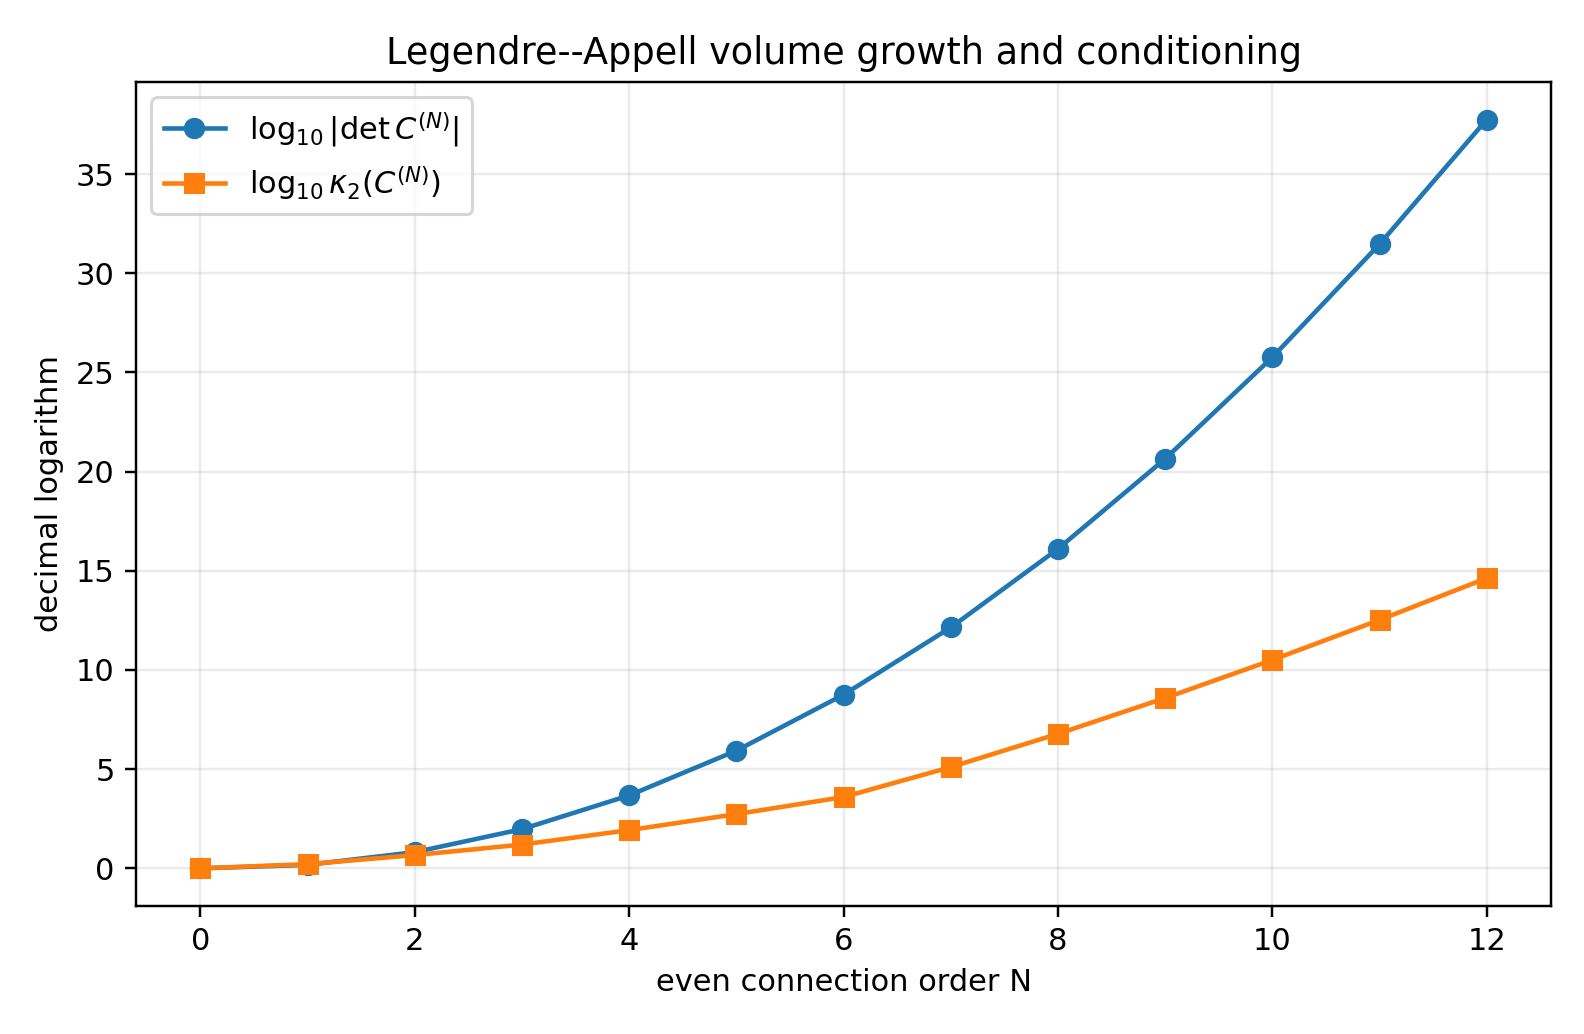
\includegraphics[width=0.92\textwidth]{appell_connection_growth.png}
\caption{Exact determinant growth and floating-point spectral condition
estimates for the even Legendre--Appell connection.  The determinant is
proved by \cref{thm:C-determinant}; condition numbers are diagnostic.}
\label{fig:appell-growth}
\end{figure}

\section{A Bernoulli-deformed Legendre operator}
\label{sec:transmutation}

\subsection{Conjugating multiplication by $x$}
Set
\begin{equation}
 K(z)=\log M_u(z),
 \qquad
 \cX=x+K'(D).
 \label{eq:Xcal}
\end{equation}
Since
\begin{equation}
 M_u(D)x=xM_u(D)+M_u'(D),
 \label{eq:commutator}
\end{equation}
we have the conjugation identity
\begin{equation}
 M_u(D)xM_u(D)^{-1}=x+\frac{M_u'(D)}{M_u(D)}=\cX.
 \label{eq:x-conjugation}
\end{equation}
Explicitly,
\begin{equation}
 K'(D)=\sum_{j\ge1}\kappa_{2j}\frac{D^{2j-1}}{(2j-1)!},
 \label{eq:Kprime}
\end{equation}
so the deformation is governed term-by-term by Bernoulli numbers.  The
canonical commutator remains
\begin{equation}
 [D,\cX]=1.
 \label{eq:canonical-commutator}
\end{equation}

\subsection{Transmuted recurrence and differential equation}
Recall $Q_n=M_u(D)P_n$.

\begin{theorem}[Rvachev-transmuted Legendre system]
\label{thm:transmuted}
The polynomials $Q_n$ satisfy
\begin{equation}
 Q_0=1,
 \qquad Q_1=x,
 \label{eq:Q-initial}
\end{equation}
and the operator recurrence
\begin{equation}
 \boxed{
 (n+1)Q_{n+1}=(2n+1)\cX Q_n-nQ_{n-1}.}
 \label{eq:Q-recurrence}
\end{equation}
They also satisfy the nonlocal differential equation
\begin{equation}
 \boxed{
 \left[(1-\cX^2)D^2-2\cX D+n(n+1)\right]Q_n=0.}
 \label{eq:Q-differential}
\end{equation}
For even index,
\begin{equation}
 Q_{2m}(x)=\sum_{r=0}^{m}C_{m,r}x^{2r},
 \label{eq:Q-C}
\end{equation}
so \eqref{eq:Q-recurrence} generates the connection matrix without separately
expanding Legendre polynomials.
\end{theorem}

\begin{proof}
Apply $M_u(D)$ to the classical recurrence
\[
 (n+1)P_{n+1}=(2n+1)xP_n-nP_{n-1}
\]
and use \eqref{eq:x-conjugation}.  Likewise conjugate the Legendre equation
$[(1-x^2)D^2-2xD+n(n+1)]P_n=0$.  Conjugation is an algebra homomorphism and
$D$ commutes with $M_u(D)$, giving \eqref{eq:Q-differential}.  Finally,
\eqref{eq:Q-C} is the definition of $C_{m,r}$ in the proof of
Theorem~\ref{thm:C-transform}.
\end{proof}

\begin{remark}[Bispectral interpretation]
The ordinary Legendre family is simultaneously controlled by a three-term
recurrence in degree and a second-order differential operator in $x$.
Theorem~\ref{thm:transmuted} preserves this architecture after replacing
multiplication by $x$ with the infinite-order operator $\cX$.  On each finite
polynomial space the series truncates, so all identities are algebraic.  A
natural frontier question is whether this system admits a useful nonlocal
orthogonality or a bispectral interpretation beyond formal conjugacy.
\end{remark}

\section{Legendre moments completed by a Thue--Morse row}
\label{sec:biorthogonal}

\subsection{Endpoint atoms on the physical interval}
For fixed $d$, define
\begin{equation}
 \Psi_{d,r}(x)=\frac1{2^d}
 u\!\left(\frac{x+1-2k_{d,r}}{2^{d+1}}\right),
 \qquad0\le r\le d+1.
 \label{eq:Psi}
\end{equation}
These functions form a basis of the $(d+2)$-dimensional local up-space on
$[-1,1]$.  Let
\begin{equation}
 (\mathsf L_d)_{n,r}=\frac{2n+1}{2}
 \int_{-1}^{1}\Psi_{d,r}(x)P_n(x)\Differential x,
 \qquad0\le n\le d.
 \label{eq:L-matrix}
\end{equation}
Thus $\mathsf L_d\bm b$ records the first $d+1$ Legendre coefficients of the
up-spline $\sum_rb_r\Psi_{d,r}$.

\subsection{The augmented square transform}
Define
\begin{equation}
 \cQ_d=
 \begin{pmatrix}
 \mathsf L_d\\[0.2em]
 \tau_d^{\mathsf T}
 \end{pmatrix},
 \label{eq:Q-augmented}
\end{equation}
where $\tau_d$ is \eqref{eq:tau-row}.

\begin{theorem}[Legendre--Thue--Morse biorthogonal completion]
\label{thm:augmented-invertible}
The matrix $\cQ_d\in\RealNumbers^{(d+2)\times(d+2)}$ is invertible.  If
$\bm\beta_{d;n}$ is the endpoint coordinate vector of $P_n$, then
\begin{equation}
 \cQ_d\bm\beta_{d;n}=
 \begin{pmatrix}\bm e_n\\0\end{pmatrix},
 \qquad0\le n\le d.
 \label{eq:Q-beta}
\end{equation}
Consequently the first $d+1$ columns of $\cQ_d^{-1}$ are precisely
$\bm\beta_{d;0},\ldots,\bm\beta_{d;d}$.  The last column
$\bm\delta_d=\cQ_d^{-1}\bm e_{d+1}$ is characterized by
\begin{equation}
 \mathsf L_d\bm\delta_d=0,
 \qquad
 \tau_d^{\mathsf T}\bm\delta_d=1.
 \label{eq:defect-column}
\end{equation}
Its synthesized function is the unique normalized nonpolynomial direction
whose first $d+1$ Legendre moments vanish.
\end{theorem}

\begin{proof}
Suppose $\cQ_d\bm b=0$.  The last row gives
$\tau_d^{\mathsf T}\bm b=0$, so the synthesis
$f=\sum_rb_r\Psi_{d,r}$ is a polynomial in $\Pi_d$ by the exact
polynomiality certificate.  The first $d+1$ rows say that every Legendre
coefficient of $f$ through degree $d$ is zero.  Hence $f=0$.  Because the
$\Psi_{d,r}$ form a basis, $\bm b=0$.  Thus $\cQ_d$ is invertible.
For the endpoint vector of $P_n$, orthogonality and polynomiality give
\[
 \mathsf L_d\bm\beta_{d;n}=\bm e_n,
 \qquad \tau_d^{\mathsf T}\bm\beta_{d;n}=0,
\]
which proves \eqref{eq:Q-beta}.  The final assertion is the definition of the
last inverse column.
\end{proof}

\begin{resultbox}
\textbf{Interpretation.}
The $d+1$ ordinary Legendre moment rows cannot distinguish the one-dimensional
nonpolynomial defect inside the local $(d+2)$-dimensional up-space.  A single
finite Thue--Morse row completes them to an invertible coordinate transform.
The inverse contains both the complete polynomial synthesis table and the
canonical defect coordinate.
\end{resultbox}

\subsection{Dyadic Fabius cell moments}
For $d\ge2$, all endpoint atoms in \eqref{eq:Psi} sample the left half of the
support.  Set
\begin{equation}
 a=d+1-r,
 \qquad M=2^d.
 \label{eq:a-cell}
\end{equation}
A change of variables followed by \eqref{eq:F-up} gives
\begin{equation}
 \boxed{
 (\mathsf L_d)_{n,r}
 =(2n+1)\int_{a/M}^{(a+1)/M}
 F(s)P_n\!\left(2Ms-(2a+1)\right)\Differential s.}
 \label{eq:F-cell-matrix}
\end{equation}

\begin{proof}
In \eqref{eq:L-matrix}, put
$y=(x+1-2k_{d,r})/(2M)$.  The factor $M^{-1}$ in $\Psi_{d,r}$ and
$\Differential x=2M\Differential y$ leave a factor $2$, which cancels the $1/2$ in the Legendre
normalization.  The integration interval is
$[-k_{d,r}/M,(1-k_{d,r})/M]$.  With $s=y+1$ it becomes
$[a/M,(a+1)/M]$, and
$x=2Ms-(2a+1)$.
\end{proof}

Equation \eqref{eq:F-cell-matrix} is a particularly concrete closure of the
conceptual loop: the inverse of a matrix of adjacent dyadic Fabius cell
moments, completed by one Thue--Morse row, gives the coefficients of Legendre
polynomials in a finite up-atom dictionary.  Polynomial expansion of $P_n$,
followed by the repository's polynomial-weighted integration identities,
reduces these entries to exact dyadic Fabius data.

\section{Arithmetic and $q$-structural consequences}
\label{sec:arithmetic}

\subsection{Rationality at every layer}
The following quantities are rational:
\begin{itemize}
\item the moments $\mu_{2m}$ and reciprocal moments $\gamma_{2m}$;
\item the connection coefficients $C_{m,r}$ and $D_{r,m}$;
\item every endpoint coefficient $\beta_{d;n,r}$;
\item the Fourier--Legendre coefficients $\lambda_{2m}$;
\item every finite closed-loop coefficient $B_{N,r}$.
\end{itemize}
The reasons are mutually reinforcing: Bernoulli cumulants generate moments
and reciprocal moments by Bell recurrences; dyadic Fabius values are rational;
the endpoint multiplier $H_d$ has rational coefficients; and the
$q$-integer triangular solve has integer entries and unit diagonal.

\subsection{Three appearances of the same dyadic arithmetic}
Three polynomial products occur in apparently different roles:
\begin{enumerate}
\item the infinite sinc product controls zero multiplicities through
$1+\TwoAdicValuation(m)$;
\item the finite alias annihilator is the $q$-integer product
$\mathfrak A_d(z)=\prod_{m=1}^d[2^m]_z$;
\item multiplying by $(z-1)^{d+1}$ turns it into the finite Thue--Morse
product \eqref{eq:tm-factor}.
\end{enumerate}
The first chooses the scale $2^d$, the second removes exponentially many
alias degrees of freedom, and the third identifies the single obstruction to
polynomiality after restriction.  The same chain is present inside the
Legendre formulas because Algorithm~\ref{alg:endpoint} is applied to
$P_n(2t-1)$ without alteration.

\subsection{A $q$-binomial form of the connection coefficients}
Combining \eqref{eq:C-explicit} with \eqref{eq:moment-Fabius} yields
\begin{align}
 C_{m,r}
 &=\frac{2^{1-2m}}{(2r)!}
 \sum_{j=r}^{m}(-1)^{m-j}
 \frac{(2m+2j)!}{(m-j)!(m+j)!}\notag\\
 &\hspace{26mm}\times
 2^{\binom{2(j-r)+1}{2}}
 F\!\left(2^{-2(j-r)-1}\right).
 \label{eq:C-Fabius}
\end{align}
The repository expresses the dyadic values in terms of Gaussian binomial and
$q$-Pochhammer data.  Substituting those formulas into
\eqref{eq:C-Fabius} produces a finite $q=1/2$ representation of the complete
Legendre--Appell matrix.  A useful unsolved problem is to resum the nested
finite sums into a single terminating basic hypergeometric expression.

\subsection{Denominators and valuations}
The exact data show two distinct sources of denominator growth:
Bernoulli/Bell denominators in $H_d$ and the rational Legendre/Fabius moment
coefficients.  The $q$-integer solve itself introduces no division.  This
suggests studying odd-prime support separately from $2$-adic valuation.
Von Staudt--Clausen controls the Bernoulli primes, while the dyadic factors are
governed by the explicit powers in \eqref{eq:moment-Fabius} and by cancellation
against $\mathfrak A_d(1)=2^{d(d+1)/2}$.

\section{Conditioning, endpoint flatness, and Lambert--$W$}
\label{sec:conditioning}

\subsection{Exact identities versus unstable evaluation}
The endpoint formulas place all sample arguments in a boundary layer whose
width is comparable with
\begin{equation}
 \delta_d\asymp\frac{d}{2^d}.
 \label{eq:delta-d}
\end{equation}
Because $u(-1+s)=F(s)$ is flat at $s=0$, the atom values are extremely small,
whereas their rational coefficients are extremely large.  Cancellation is
therefore intrinsic to the right-endpoint basis.

The exact data through degree $12$ are summarized in
\cref{fig:endpoint-growth}.  For the raw coefficient vector of the
degree-matched $P_d$ formula,
\begin{equation}
 \log_{10}\max_r|\beta_{d;d,r}|
 =2.27,\ 7.24,\ 13.86,\ 21.92,\ 31.43,\ 42.32
 \label{eq:beta-data}
\end{equation}
for $d=2,4,6,8,10,12$, respectively.

\begin{figure}[htbp]
\centering
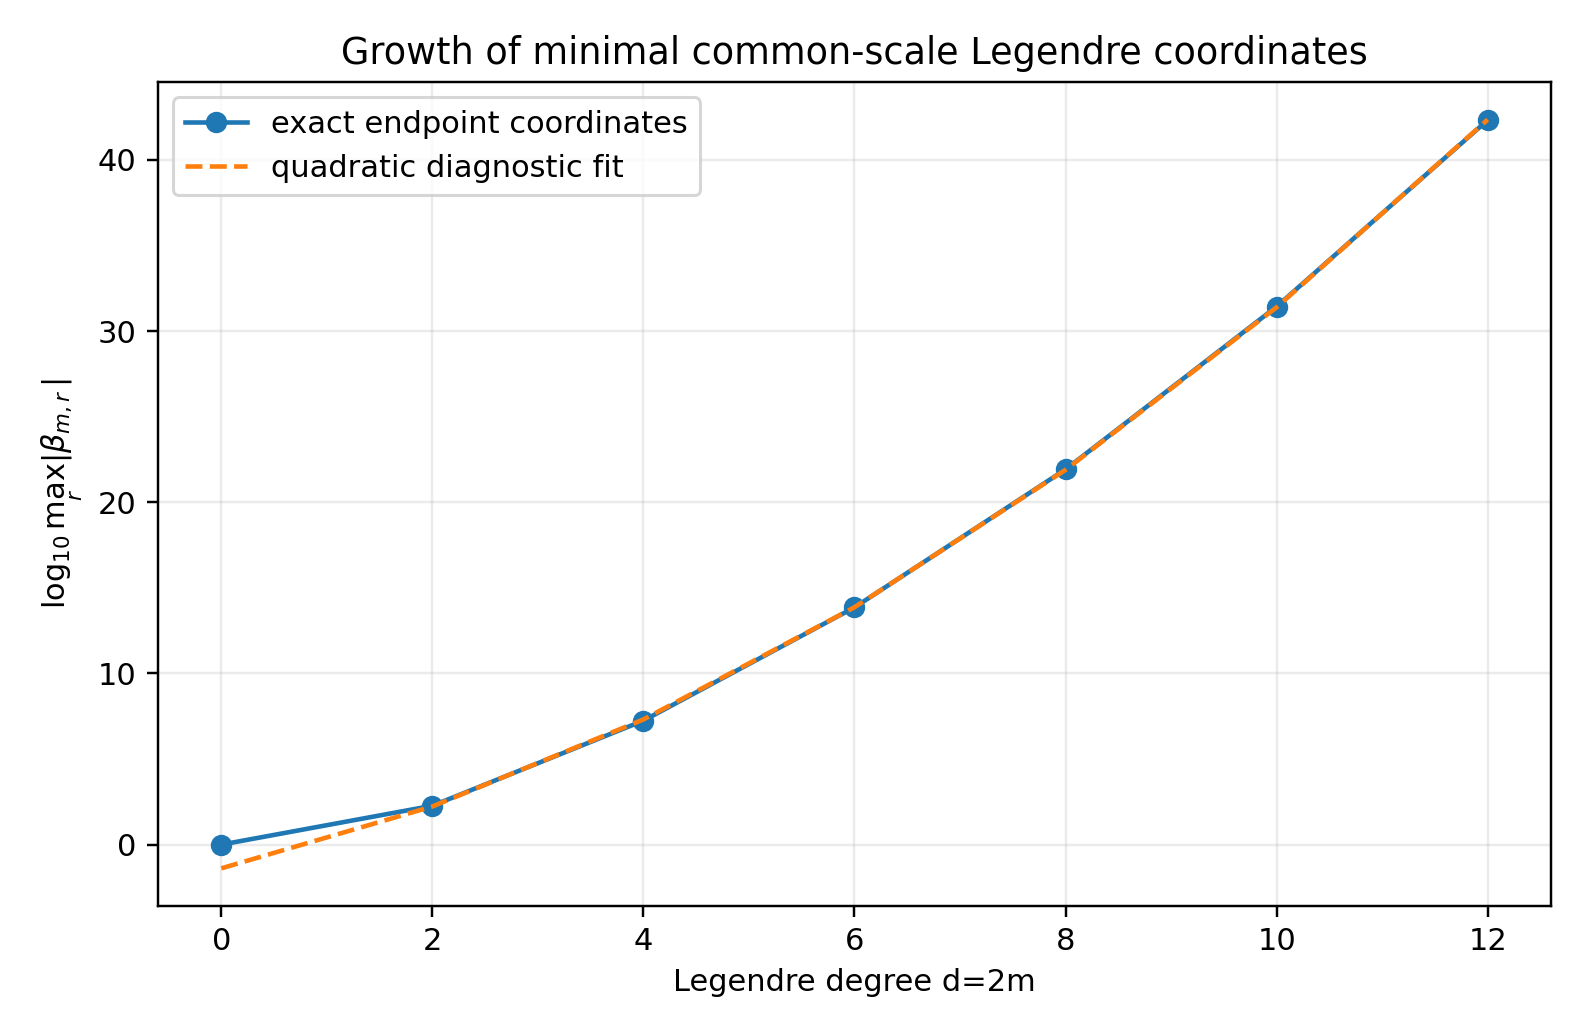
\includegraphics[width=0.92\textwidth]{endpoint_coefficient_growth.png}
\caption{Exact rational endpoint-coordinate growth for the degree-matched
even Legendre polynomials.  The dashed curve is only a diagnostic quadratic
fit, not a proved asymptotic.}
\label{fig:endpoint-growth}
\end{figure}

\subsection{Closed-loop coefficient growth}
For the one-scale partial-sum coefficients $B_{N,r}$, exact computation gives
\begin{table}[htbp]
\centering
\caption{One-scale closed-loop coordinate growth.  ``Separate-scale
occurrences'' is $(N+1)(N+2)$.}
\label{tab:fixed-summary}
\resizebox{\textwidth}{!}{% Generated exactly by legendre_rvachev_experiments.py
\begin{tabular}{@{}rrrrrr@{}}
\toprule
$N$ & degree & atoms & separate-scale occurrences & $\log_{10}\max|B_{N,r}|$ & bits\\
\midrule
0 & 0 & 2 & 2 & -0.301 & 2\\
1 & 2 & 4 & 6 & 2.181 & 11\\
2 & 4 & 6 & 12 & 6.787 & 34\\
3 & 6 & 8 & 20 & 12.319 & 64\\
4 & 8 & 10 & 30 & 20.851 & 104\\
5 & 10 & 12 & 42 & 30.023 & 156\\
6 & 12 & 14 & 56 & 40.741 & 217\\
\bottomrule
\end{tabular}
}
\end{table}

\begin{figure}[htbp]
\centering
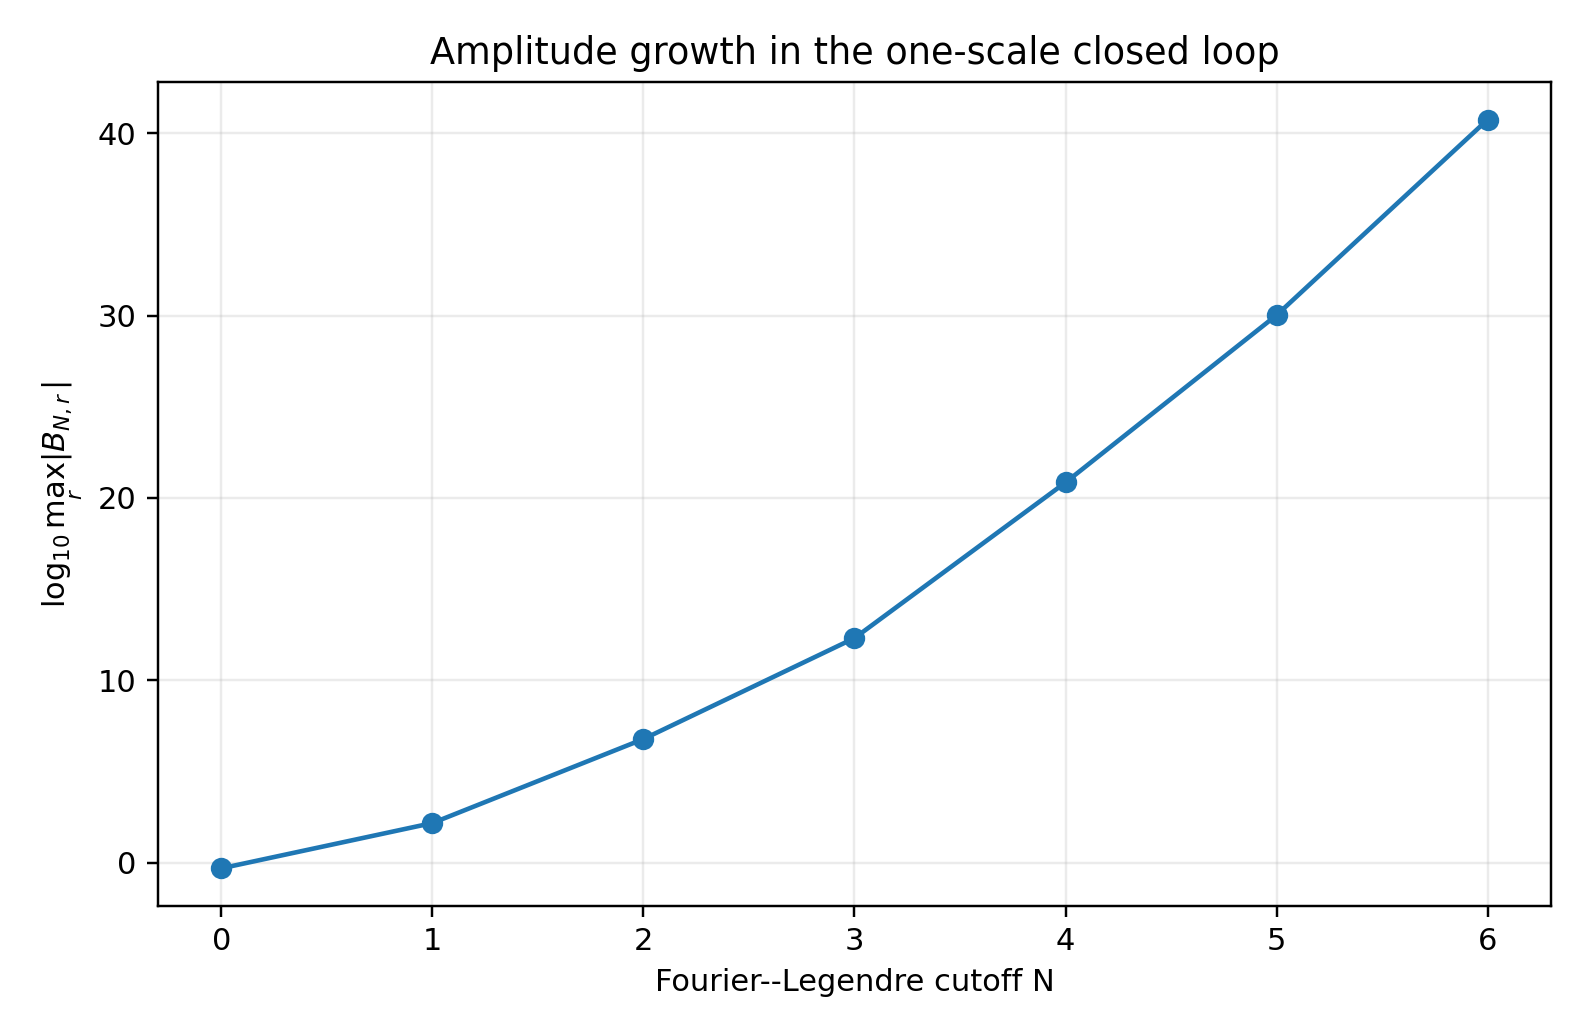
\includegraphics[width=0.88\textwidth]{fixed_scale_loop_coefficients.png}
\caption{Maximum exact coordinate magnitude in the one-scale closed loop.
The plotted values are decimal logarithms of exact rationals.}
\label{fig:loop-growth}
\end{figure}

The atom count is linear, but coefficient complexity is not.  At $N=6$, only
$14$ atoms remain after compression, while the largest raw coefficient has
about $41$ decimal digits and the largest numerator or denominator requires
$217$ bits.

\subsection{Why Lambert--$W$ appears}
The repository's sharp endpoint analysis reduces the small-$s$ behavior of
$F(s)$ to a saddle equation whose inversion uses a branch of Lambert--$W$.
At the endpoint scale \eqref{eq:delta-d},
\begin{equation}
 \log\frac1{\delta_d}=d\log2-\log d+\BigO(1).
 \label{eq:log-delta}
\end{equation}
The leading flat-tail law is quadratic in this logarithm, with lower-order
$\log\log(1/s)$ and periodic dyadic corrections.  Independently, the
triangular algorithm contains the mass
$\mathfrak A_d(1)=2^{d(d+1)/2}$.  Heuristically, one quadratic contribution
comes from this finite convolution law and another from compensating the flat
endpoint values.  This explains why the observed natural logarithm of the
largest coefficient is close to a constant times $d^2$, and motivates the
sharp conjecture in \cref{conj:growth}.

This heuristic must not be mistaken for a proof.  A proof would require a
uniform saddle analysis of a signed finite combination, not merely a pointwise
asymptotic for $F$.

\subsection{Numerical diagnostic}
A finite-convolution approximation of $u$ was used only to visualize the
low-degree formulas.  The maximum residuals on a 501-point grid were roughly
$7.6\times10^{-6}$, $9.9\times10^{-5}$, and $1.2\times10^{-3}$ for
$P_0,P_2,P_4$.  The corresponding maximum cancellation ratios were about
$1$, $3.6\times10^4$, and $4.7\times10^8$.

\begin{figure}[htbp]
\centering
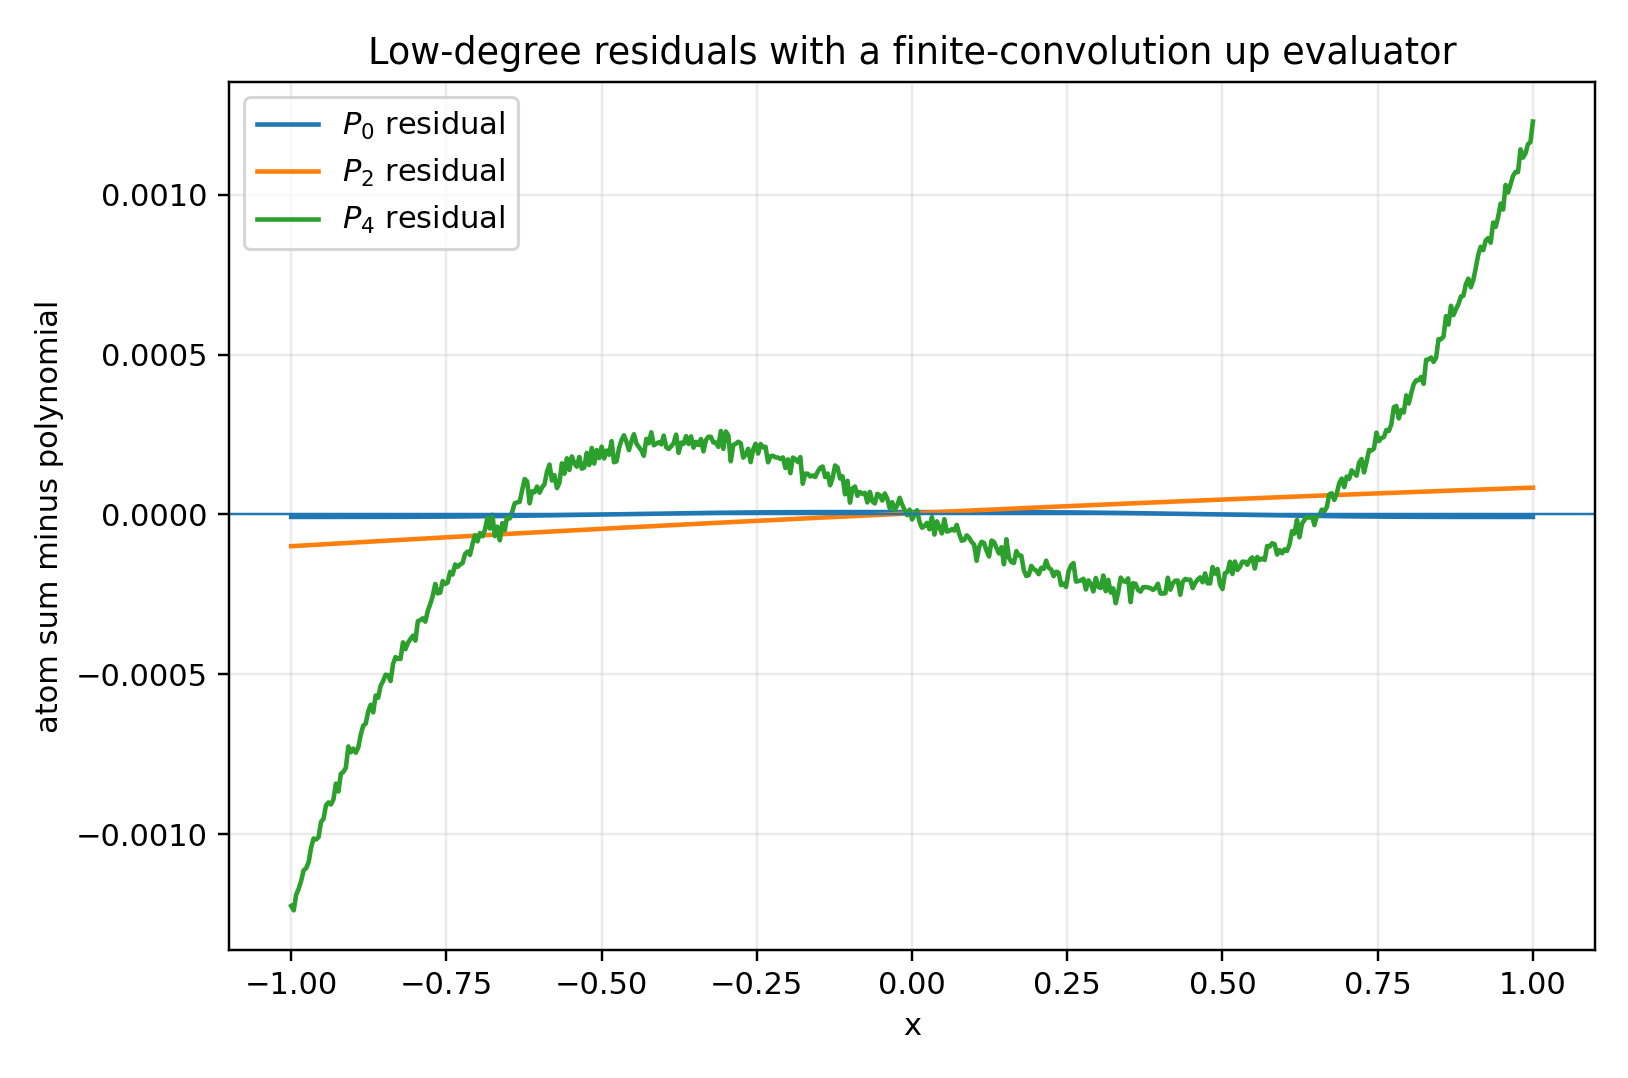
\includegraphics[width=0.91\textwidth]{low_degree_atom_reconstruction.png}
\caption{Floating-point residuals obtained from a finite-convolution
approximation of $u$.  The exact symbolic identities have zero residual; the
plot measures evaluator and cancellation error.}
\label{fig:reconstruction}
\end{figure}

\section{Further deductions from the closed loop}
\label{sec:deductions}

\subsection{A finite-rank extension/restriction factorization}
Let $R_d$ restrict a function to its first $d+1$ Legendre coefficients, and
let $E_d$ map a polynomial coefficient vector to the endpoint up-spline with
coordinates supplied by $\cQ_d^{-1}$.  Then on $\Pi_d$,
\begin{equation}
 R_dE_d=I.
 \label{eq:right-inverse}
\end{equation}
Thus $E_dR_d$ is a finite-rank projection on the local up-space.  The
polynomial subspace is selected not by point sampling but by Legendre moments,
and the extra defect coordinate is selected by Thue--Morse.  This gives a
basis-free interpretation of the endpoint construction.

\subsection{A defect-sensitive reconstruction formula}
For any local endpoint up-spline
$f=\sum_rb_r\Psi_{d,r}$, define
\begin{equation}
 \alpha_n=\frac{2n+1}{2}\int_{-1}^{1}f(x)P_n(x)\Differential x,
 \qquad
 \eta=\tau_d^{\mathsf T}\bm b.
 \label{eq:alpha-eta}
\end{equation}
Then
\begin{equation}
 \bm b=\cQ_d^{-1}
 \begin{pmatrix}\alpha_0\\ \vdots\\ \alpha_d\\ \eta\end{pmatrix}.
 \label{eq:full-reconstruction}
\end{equation}
Hence the local up-spline is determined by $d+1$ classical moments plus one
digital certificate.  Polynomial synthesis is the special case $\eta=0$.
This is an exact finite analogue of augmenting an incomplete moment problem by
one boundary datum.

\subsection{Universality beyond the Rvachev law}
The direct connection theorem has a universal component.  Given any normalized
even moment series $M(z)$, define its Appell family by $\EulerE^{xz}/M(z)$.  The
formulas \eqref{eq:C-moment}, \eqref{eq:D-explicit}, and
\eqref{eq:C-det} remain valid with the new moments and reciprocal moments.
What is special to Rvachev is not the triangular Appell algebra but the finite
realization of those Appell coordinates by compactly supported dyadic atoms,
the $q$-integer alias annihilator, and the Thue--Morse defect row.

\subsection{A route to fast coefficient generation}
There are now two independent recurrences:
\begin{itemize}
\item \eqref{eq:Q-recurrence} generates the Legendre--Appell rows $C_{m,r}$;
\item \eqref{eq:beta-rec} sends any polynomial row to the endpoint atom
coordinates.
\end{itemize}
Their composition gives a structured transform from Legendre coefficients to
endpoint coordinates without expanding each $P_n$ in monomials.  For a dense
polynomial of degree $d$, both stages admit quadratic arithmetic complexity.
The special three-term degree recurrence suggests that subquadratic algorithms
may be possible using divide-and-conquer polynomial arithmetic and Toeplitz
convolution.

\section{Conjectures and frontier directions}
\label{sec:conjectures}

\begin{conjecture}[Strict endpoint alternation]
\label{conj:alternation}
For every $m\ge1$, the degree-matched right-endpoint coordinates of $P_{2m}$
satisfy
\begin{equation}
 \boxed{(-1)^r\beta_{2m;2m,r}>0,
 \qquad0\le r\le2m+1.}
 \label{eq:alternation-conj}
\end{equation}
Exact computation verifies this through $m=6$.  A proof may follow from a
total-positivity or extended-Chebyshev property of the endpoint atom system,
but no such theorem is presently available for these flat nonanalytic atoms.
\end{conjecture}

\begin{conjecture}[Quadratic logarithmic endpoint growth]
\label{conj:growth}
Let
$\mathfrak B_d=\max_r|\beta_{d;d,r}|$ for even $d$.  Then
\begin{equation}
 \boxed{
 \lim_{\substack{d\to\infty\\2\mid d}}
 \frac{\log\mathfrak B_d}{d^2}=\log2.}
 \label{eq:beta-growth-conj}
\end{equation}
The same leading constant is expected for
$\max_r|B_{N,r}|$ after writing $d=2N$, at least along a limsup.  The proposed
constant reflects the combined $q$-integer mass and flat-tail compensation;
Lambert--$W$ and dyadic periodic corrections should enter the lower-order
terms.
\end{conjecture}

\begin{conjecture}[Legendre--Fabius augmented determinant]
\label{conj:augdet}
After a natural diagonal normalization of the Legendre rows and the endpoint
atoms, the determinant of $\cQ_d$ factors into a product of powers of two,
short $q$-integer factors, and a residual determinant with controlled odd
prime support.  Equivalently, the inverse table of all Legendre endpoint
coordinates should admit a fraction-free elimination governed by the same
cyclotomic factors as $\mathfrak A_d$.
\end{conjecture}

\begin{conjecture}[Total positivity after checkerboard scaling]
\label{conj:total-positivity}
There exists a canonical ordering and positive diagonal scaling of the
right-endpoint atom evaluation or moment matrix for which checkerboard sign
changes convert the relevant Legendre synthesis minors to nonnegative
minors.  Strict positivity of the maximal minors would imply
Conjecture~\ref{conj:alternation} and a variation-diminishing property for
polynomial endpoint coordinates.
\end{conjecture}

\begin{problem}[$q$-hypergeometric compression]
Insert the repository's Gaussian-binomial formulas for
$F(2^{-2s-1})$ into \eqref{eq:C-Fabius}.  Can the resulting double finite sum
be expressed as one terminating ${}_r\phi_s$ series, a $q$-Racah-type
connection coefficient, or a determinant of Gaussian binomial entries?  Such
a formula could expose hidden orthogonality in the index pair $(m,r)$.
\end{problem}

\begin{problem}[Nonlocal orthogonality of the transmuted system]
Find a bilinear form, positive if possible, for which the polynomials
$Q_n=M_u(D)P_n$ are orthogonal and the operator in
\eqref{eq:Q-differential} is symmetric.  Formal conjugacy transports the
Legendre inner product to
\begin{equation}
 \langle f,g\rangle_u
 =\int_{-1}^{1}\bigl[M_u(D)^{-1}f\bigr](x)
                 \bigl[M_u(D)^{-1}g\bigr](x)\Differential x,
 \label{eq:formal-inner-product}
\end{equation}
but locality, positivity on suitable completions, and a spectral theorem are
nontrivial.
\end{problem}

\begin{problem}[Parity-adapted fixed dictionaries]
The even polynomial space of degree at most $2N$ has dimension $N+1$, whereas
the full endpoint dictionary has $2N+2$ atoms.  Can one construct $N+1$
symmetric atom pairs or other parity-adapted blocks that form a fixed basis of
the even subspace and improve conditioning?  The count should be compared in
blocks, raw atom occurrences, support overhang, and coefficient norm.
\end{problem}

\begin{problem}[Condition-optimal common-scale basis]
Among all $(d+2)$-subsets of the active dyadic dictionary, minimize a
stability functional such as
\begin{equation}
 \sup_{\|p\|_\infty\le1}\|\bm b(p)\|_1,
 \qquad
 \kappa_2(\cQ_d),
 \quad\text{or}\quad
 \max_r\operatorname{dist}(\SupportOperator\Psi_{d,r},[-1,1]).
 \label{eq:basis-objectives}
\end{equation}
The right-endpoint basis is algebraically canonical but strongly
ill-conditioned.  Central consecutive bases and symmetric hybrids are the
first candidates.
\end{problem}

\begin{problem}[Sharp Lambert--$W$ coefficient asymptotics]
Combine the exact triangular formula \eqref{eq:beta-rec} with the repository's
sharp endpoint expansion for $F$, including its periodic dyadic correction.
Determine
\begin{equation}
 \log\mathfrak B_d-(\log2)d^2
 \label{eq:beta-residual}
\end{equation}
through the $d\log d$, $d$, $\log d$, and bounded periodic terms.  The main
technical obstacle is controlling cancellation among neighboring endpoint
samples uniformly in the triangular solve.
\end{problem}

\begin{problem}[Two-adic and odd-prime valuations]
For fixed index ratios $r/d$, determine asymptotic or exact formulas for
$v_2(\beta_{d;d,r})$ and for the odd denominator support.  Separate the
Bernoulli contribution, the Fabius moment contribution, and cancellation in
the integer $q$-filter.  The result should be compared with the prime support
of Gaussian binomial coefficients at $q=1/2$.
\end{problem}

\begin{problem}[Beyond base two]
For base-$b$ atomic functions, replace the sinc product, $2$-adic zero
multiplicity, and Thue--Morse product by their base-$b$ analogues.  Determine
the corresponding Legendre endpoint dictionary, digit-character certificate,
and Appell-transmuted recurrence.  The determinant
\eqref{eq:C-det} remains universal, while the finite atomic realization should
encode the new base.
\end{problem}

\begin{problem}[Formal verification]
A compact formalization path is:
\begin{enumerate}
\item import the arbitrary-polynomial endpoint theorem and its $H_d$ algorithm;
\item formalize the affine specialization in Theorem~\ref{thm:legendre-endpoint};
\item formalize the finite substitution in Theorem~\ref{thm:finite-loop};
\item prove the moment formulas for $C$ and $D$ by finite sums;
\item verify the triangular determinant and the conjugated recurrence; and
\item formalize the kernel argument for Theorem~\ref{thm:augmented-invertible}.
\end{enumerate}
All steps after the imported analytic lemmas are finite polynomial or matrix
algebra.
\end{problem}

\section{Conclusion}
The arbitrary-polynomial endpoint theorem has a particularly clean Legendre
specialization.  Every $P_n$ is exactly a finite linear combination of shifts
of one common dyadic dilate of Rvachev's up-function.  At a Fourier--Legendre
cutoff, all even Legendre terms can be moved to one maximal-degree dictionary,
so the full partial sum collapses to $2N+2$ atoms.  Since the partial sums
converge uniformly, this gives a closed self-representation of $u$ by moving
finite one-scale atom systems.

The direct Legendre--Appell transform reveals a second layer.  Moment
convolution sends $P_{2m}$ to a polynomial whose monomial coefficients are the
Appell coordinates.  The forward and inverse matrices are explicit finite
Bernoulli--Bell transforms; their determinant is universal and depends only
on the leading Legendre coefficients.  Conjugating the Legendre operators by
the moment series replaces $x$ with the Bernoulli differential position
operator $x+(\log M_u)'(D)$.

The endpoint coordinates admit a complementary moment interpretation.  The
matrix of the first $d+1$ Legendre moments of the $d+2$ endpoint atoms is one
row short of being square.  The missing row is exactly the finite
Thue--Morse polynomiality certificate.  Its inverse simultaneously produces
all Legendre synthesis vectors and the unique normalized nonpolynomial defect.
This is the most compact structural form of the loop: classical orthogonal
moments are completed by one digital row arising from the same dyadic product
that controls the sinc zeros and $q$-integer aliases.

The representation is exact but numerically delicate.  Linear atom counts
coexist with quadratic-logarithmic coefficient growth because the atoms are
sampled near a flat endpoint.  That is not a defect of the proof; it is a
geometric feature connecting endpoint asymptotics, Lambert--$W$, Thue--Morse
cancellation, and the arithmetic of dyadic Fabius values.  The most promising
next steps are a sharp saddle analysis of the coefficient envelope, a
checkerboard total-positivity theorem, a condition-optimal central dictionary,
and a $q$-hypergeometric formula for the Legendre--Appell matrix.

\appendix

\section{Formula sheet}

\paragraph{Moment and Appell data.}
\begin{align*}
 M_u(z)&=\prod_{j\ge1}\frac{\sinh(z/2^j)}{z/2^j},
 &\kappa_{2m}&=\frac{B_{2m}}{2m(1-4^{-m})},\\
 \frac1{M_u(z)}&=\sum_{n\ge0}\gamma_n\frac{z^n}{n!},
 &\frac{\EulerE^{xz}}{M_u(z)}&=\sum_{n\ge0}A_n(x)\frac{z^n}{n!}.
\end{align*}

\paragraph{Endpoint dictionary.}
\begin{align*}
 M&=2^d,& k_{d,r}&=M-d-1+r,\\
 \Psi_{d,r}(x)&=2^{-d}u\!\left(\frac{x+1-2k_{d,r}}{2^{d+1}}\right),
 &0&\le r\le d+1.
\end{align*}

\paragraph{Coefficient algorithm.}
\begin{align*}
 H_d(z)&=\left(\frac{z}{2\sinh(z/2)}\right)^d\frac1{M_u(z)},\\
 \mathfrak A_d(z)&=\prod_{m=1}^d[2^m]_z=\sum_ja_{d,j}z^j,\\
 g_r&=2^{d(d+1)/2}[H_d(D)P](r-d/2),\\
 b_0&=g_0,
 &b_r&=g_r-\sum_{s<r}a_{d,r-s}b_s.
\end{align*}

\paragraph{Legendre endpoint formula.}
\[
 P_n(x)=2^{-d}\sum_{r=0}^{d+1}\beta_{d;n,r}
 u\!\left(\frac{x+1-2(2^d-d-1+r)}{2^{d+1}}\right).
\]

\paragraph{One-scale closed loop.}
\begin{align*}
 B_{N,r}&=\sum_{m=0}^N\lambda_{2m}\beta_{2N;2m,r},\\
 S_N(x)&=4^{-N}\sum_{r=0}^{2N+1}B_{N,r}
 u\!\left(\frac{x+1-2(4^N-2N-1+r)}{2\cdot4^N}\right),\\
 u(x)&=\lim_{N\to\infty}S_N(x)\quad\text{uniformly on }[-1,1].
\end{align*}

\paragraph{Legendre--Appell connection.}
\begin{align*}
 P_{2m}&=\sum_{r=0}^mC_{m,r}A_{2r},
 &C_{m,r}&=[x^{2r}]M_u(D)P_{2m},\\
 A_{2r}&=\sum_{m=0}^rD_{r,m}P_{2m},
 &\det C^{(N)}&=\prod_{m=0}^N2^{-2m}\binom{4m}{2m}.
\end{align*}

\paragraph{Transmuted Legendre system.}
\begin{align*}
 Q_n&=M_u(D)P_n,&\cX&=x+(\log M_u)'(D),\\
 (n+1)Q_{n+1}&=(2n+1)\cX Q_n-nQ_{n-1},\\
 [(1-\cX^2)D^2-2\cX D+n(n+1)]Q_n&=0.
\end{align*}

\paragraph{Augmented moment matrix.}
\begin{align*}
 (\mathsf L_d)_{n,r}&=\frac{2n+1}{2}\int_{-1}^{1}\Psi_{d,r}P_n,\\
 \cQ_d&=\begin{pmatrix}\mathsf L_d\\ \tau_d^{\mathsf T}\end{pmatrix},
 &\bm\beta_{d;n}&=\cQ_d^{-1}\begin{pmatrix}\bm e_n\\0\end{pmatrix}.
\end{align*}

\section{Pseudocode for the direct closed loop}
\begin{lstlisting}[style=pseudo,caption={Exact common-scale Legendre closure.}]
INPUT: cutoff N
OUTPUT: exact rational B[0..2N+1], centers, common scale

d <- 2N
M <- 2^d
construct moments mu[0..d] from Bernoulli cumulants
construct lambda[0..N] from integral up(x) P_(2m)(x)
construct H_d(z) modulo z^(d+1)
construct a[0..d+1] from product_(j=1)^d [2^j]_z,
    truncating every convolution

for m=0..N:
    P(t) <- P_(2m)(2t-1)
    G(t) <- H_d(D_t) P(t)
    for r=0..d+1:
        g[r] <- 2^(d(d+1)/2) G(r-d/2)
        beta[m,r] <- g[r] - sum_(s<r) a[r-s] beta[m,s]

for r=0..d+1:
    B[r] <- sum_(m=0)^N lambda[2m] beta[m,r]
    k[r] <- M-d-1+r
    center[r] <- 2k[r]-1

RETURN amplitude[r]=B[r]/M,
       atom[r](x)=up((x-center[r])/(2M))

equality: S_N(x)=sum_r amplitude[r] atom[r](x), -1<=x<=1
\end{lstlisting}

\section{Reproducibility files}
The accompanying ZIP archive contains:
\begin{description}[style=nextline,leftmargin=2.4em]
\item[\path{legendre_rvachev_closed_loop.tex}]
The complete LaTeX source.
\item[\path{legendre_rvachev_closed_loop.pdf}]
The rendered report.
\item[\path{legendre_rvachev_experiments.py}]
Commented exact and numerical experiments.
\item[\path{data/legendre_appell_connection.csv}]
Exact $C$ and $D$ entries through connection order $12$.
\item[\path{data/legendre_appell_conditioning.csv}]
Exact determinants and floating-point condition estimates.
\item[\path{data/minimal_legendre_endpoint_coefficients.csv}]
Degree-matched endpoint vectors through $P_{12}$.
\item[\path{data/fixed_scale_loop_summary.csv} and
\path{data/fixed_scale_loop_coefficients.csv}]
One-scale partial-sum coordinates through cutoff $N=6$.
\item[\path{data/thue_morse_certificate_checks.csv}]
Exact certificate rows and zero residuals.
\item[\path{data/transmuted_recurrence_checks.txt}]
Exact zero residuals for the transmuted recurrence through $n=13$.
\item[\path{figures/} and \path{generated/}]
The figures and exact LaTeX fragments used in the report.
\item[\path{README.md}, \path{requirements.txt}, and \path{SHA256SUMS}]
Reproduction instructions, dependencies, and integrity hashes.
\end{description}

\begin{thebibliography}{99}

\bibitem{RepoMain}
V.~Reshetnikov,
\newblock \emph{The Fabius Function and Rvachev's Up-Function: Exact
Arithmetic, Probability, Fourier Analysis, and Corrected Sharp Asymptotics},
\newblock \Repo{} repository,
\path{Analysis/FabiusFunction/docs/Fabius_Function_and_Rvachev_Up/},
snapshot 29 August 2026,
\newblock \url{https://github.com/VladimirReshetnikov/ProveIt}.

\bibitem{RepoPoly}
V.~Reshetnikov,
\newblock \emph{Up-Function Polynomial Synthesis},
\newblock \Repo{} repository,
\path{Analysis/FabiusFunction/docs/semi-formalized-research-frontiers/drafts/representations/Up_Polynomial_Synthesis/},
snapshot 29 August 2026.

\bibitem{RepoInverse}
V.~Reshetnikov,
\newblock \emph{Inverse and Sampling Frontiers for the Fabius--Rvachev System},
\newblock \Repo{} repository,
\path{Analysis/FabiusFunction/docs/semi-formalized-research-frontiers/drafts/inverse-and-sampling/},
snapshot 29 August 2026.

\bibitem{RepoRepresentations}
V.~Reshetnikov,
\newblock \emph{Representation Frontiers for Fabius and Rvachev Functions},
\newblock \Repo{} repository,
\path{Analysis/FabiusFunction/docs/semi-formalized-research-frontiers/drafts/representations/},
snapshot 29 August 2026.

\bibitem{RepoQ}
V.~Reshetnikov,
\newblock \emph{$q$-Series and Exponent Frontiers in the Fabius--Rvachev
System},
\newblock \Repo{} repository,
\path{Analysis/FabiusFunction/docs/semi-formalized-research-frontiers/drafts/exponents-and-q-series/},
snapshot 29 August 2026.

\bibitem{Fabius1966}
J.~Fabius,
\newblock A probabilistic example of a nowhere analytic $C^\infty$-function,
\newblock \emph{Zeitschrift f"ur Wahrscheinlichkeitstheorie und Verwandte
Gebiete} \textbf{5} (1966), 173--174.

\bibitem{Arias1982}
J.~Arias de Reyna,
\newblock An infinitely differentiable function with compact support:
definition and properties,
\newblock English translation of the 1982 article, arXiv:1702.05442 (2017).

\bibitem{Arias2018}
J.~Arias de Reyna,
\newblock Arithmetic of the Fabius function,
\newblock \emph{INTEGERS} \textbf{18} (2018), Article A51;
arXiv:1702.06487.

\bibitem{Rvachev1990}
V.~A.~Rvachev,
\newblock Compactly supported solutions of functional-differential equations
and their applications,
\newblock \emph{Russian Mathematical Surveys} \textbf{45} (1990), no.~1,
87--120.

\bibitem{Szego}
G.~Szeg\H{o},
\newblock \emph{Orthogonal Polynomials},
\newblock American Mathematical Society Colloquium Publications, vol.~23,
4th ed., 1975.

\bibitem{Roman}
S.~Roman,
\newblock \emph{The Umbral Calculus},
\newblock Academic Press, 1984.

\bibitem{Comtet}
L.~Comtet,
\newblock \emph{Advanced Combinatorics},
\newblock D.~Reidel, 1974.

\bibitem{StrangFix}
G.~Strang and G.~Fix,
\newblock A Fourier analysis of the finite element variational method,
\newblock in \emph{Constructive Aspects of Functional Analysis}, Edizioni
Cremonese, 1973, 793--840.

\bibitem{Corless}
R.~M.~Corless, G.~H.~Gonnet, D.~E.~G.~Hare, D.~J.~Jeffrey, and D.~E.~Knuth,
\newblock On the Lambert $W$ function,
\newblock \emph{Advances in Computational Mathematics} \textbf{5} (1996),
329--359.

\end{thebibliography}

\end{document}
